\documentclass[a4paper,12pt,titlepage]{article}      			

\usepackage[pdftex]{graphicx}
\usepackage[headheight=15pt]{geometry} 

\usepackage{fancyhdr}
\pagestyle{fancy}
\lhead{Working with GeoNode}
\chead{}
\rhead{Practical Guideline}

\usepackage[english]{babel}									
\usepackage[utf8]{inputenc}	

\usepackage{array}
\usepackage{colortbl}

\usepackage[section]{placeins}
\usepackage{float}

%PDF hyperlinks
\usepackage[colorlinks=true,linkcolor=orange,bookmarksopen=true,bookmarksnumbered=false,pdfstartpage=2]{hyperref}


\usepackage{color}
\definecolor{orange}{rgb}{1,.5,0}


\title{Guideline on GeoNode}  
\author{Michael Wagner}      												
\date{\today}     													

\clubpenalty=4500																
\widowpenalty=10000															
\linespread{1.3}

%%-------------------------Document begins--------------------------------------------
\begin{document}             										
\maketitle                   									

\tableofcontents
\listoffigures
\newpage

\section{Introduction}

\subsection{Overview}

GeoNode is a web-based platform to share geospatial data (as well as non-spatial data). GeoNode is released as Open Source Software and supports various OGC standards such as WMS, WFS, CSW, etc. It has an active user and developer community and is constantly improved and extended. GeoNode can support organisations in implementing a Spatial Data Infrastructure from the technological point of view. In the context of OpenDRI it will help the involved organisations to share data relevant to disaster risk assessment and management in an easy and standard compliant way. Figure \ref{fig:geonode_architecture} shows the overall architecture of GeoNode.

\begin{figure}[H]
	\centering
	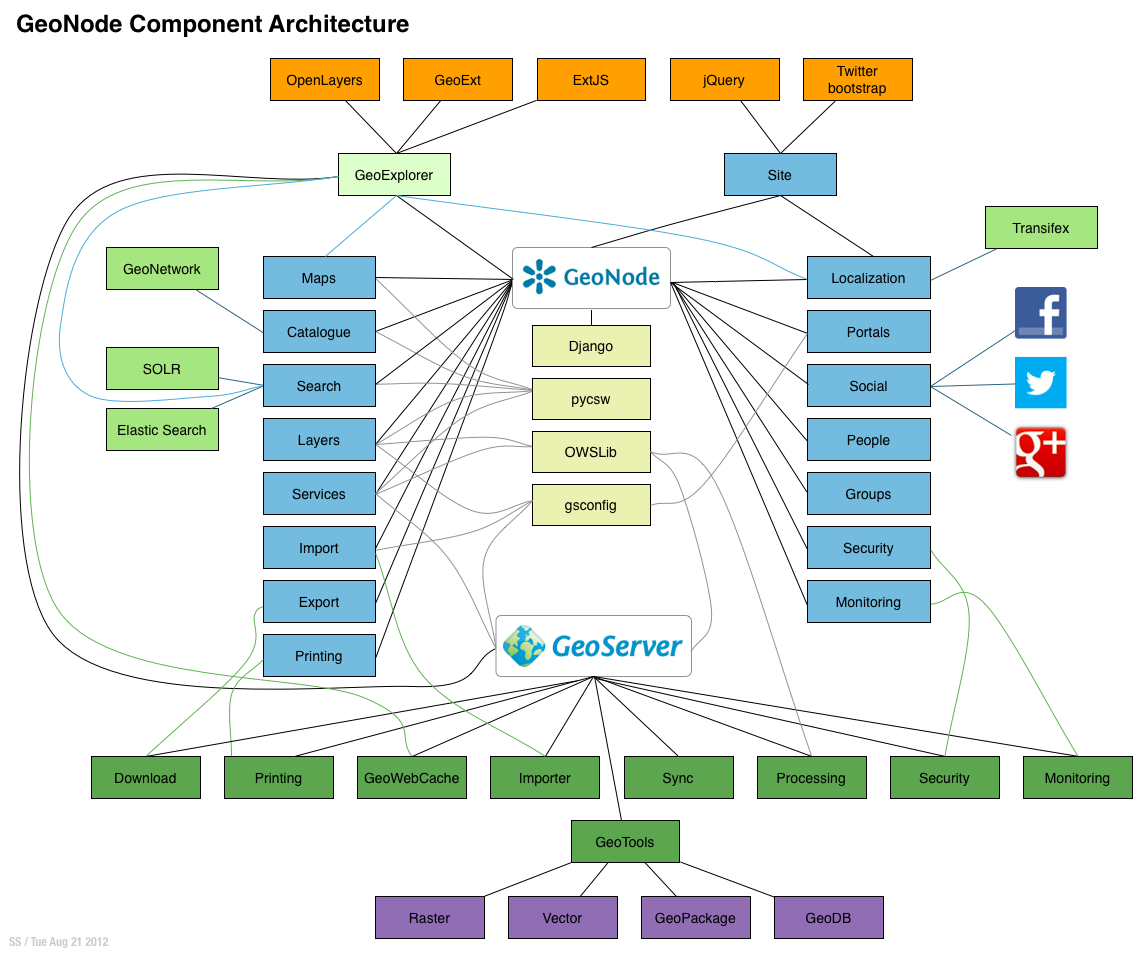
\includegraphics[width=12cm]{Images/geonode_architecture.png}
	\caption[GeoNode Architecture]{GeoNode Architecture (Source: \href{http://docs.geonode.org/en/master/tutorials/overview_and_ref/reference_doc/architecture.html}{GeoNode})}\label{fig:geonode_architecture}
\end{figure}

An pilot installation of a customised GeoNode is currently accessible under \url{http://178.63.85.21}. The underlying server hardware is hosted at a web hosting provider. Latest by the end of the project (August 2016) GeoNode should run on a government server and be accessible from within the government network.
 
The user interface of GeoNode is pretty easy to understand and utilize, there are five main sections (Figure \ref{fig:geonode_1}):
 
 \begin{itemize}
 	\item Layers: A layer is a geospatial dataset (either vector or raster). Although GeoNode supports a few file formats for data upload the most common ones are ESRI Shapefile for vector data and GeoTiff for raster data. Registered GeoNode users may upload layers and relating metadata, define layer styles, edit metadata and grant access permissions on a layer.
 	\item Maps: A map is a combination of layers and can be created and styled by registered GeoNode users.
 	\item Documents: A document can be any non-spatial dataset such as a PDF file, an image, an MS Office document, etc. Documents may be uploaded by registered GeoNode users.
 	\item People: Registered GeoNode users (having usernames and passwords)
 	\item Groups: Groups are a way to organise users. Permissions can be granted to groups and are inherited by the group members automatically.
 \end{itemize}
 
 \begin{figure}[H]
 	\centering
 	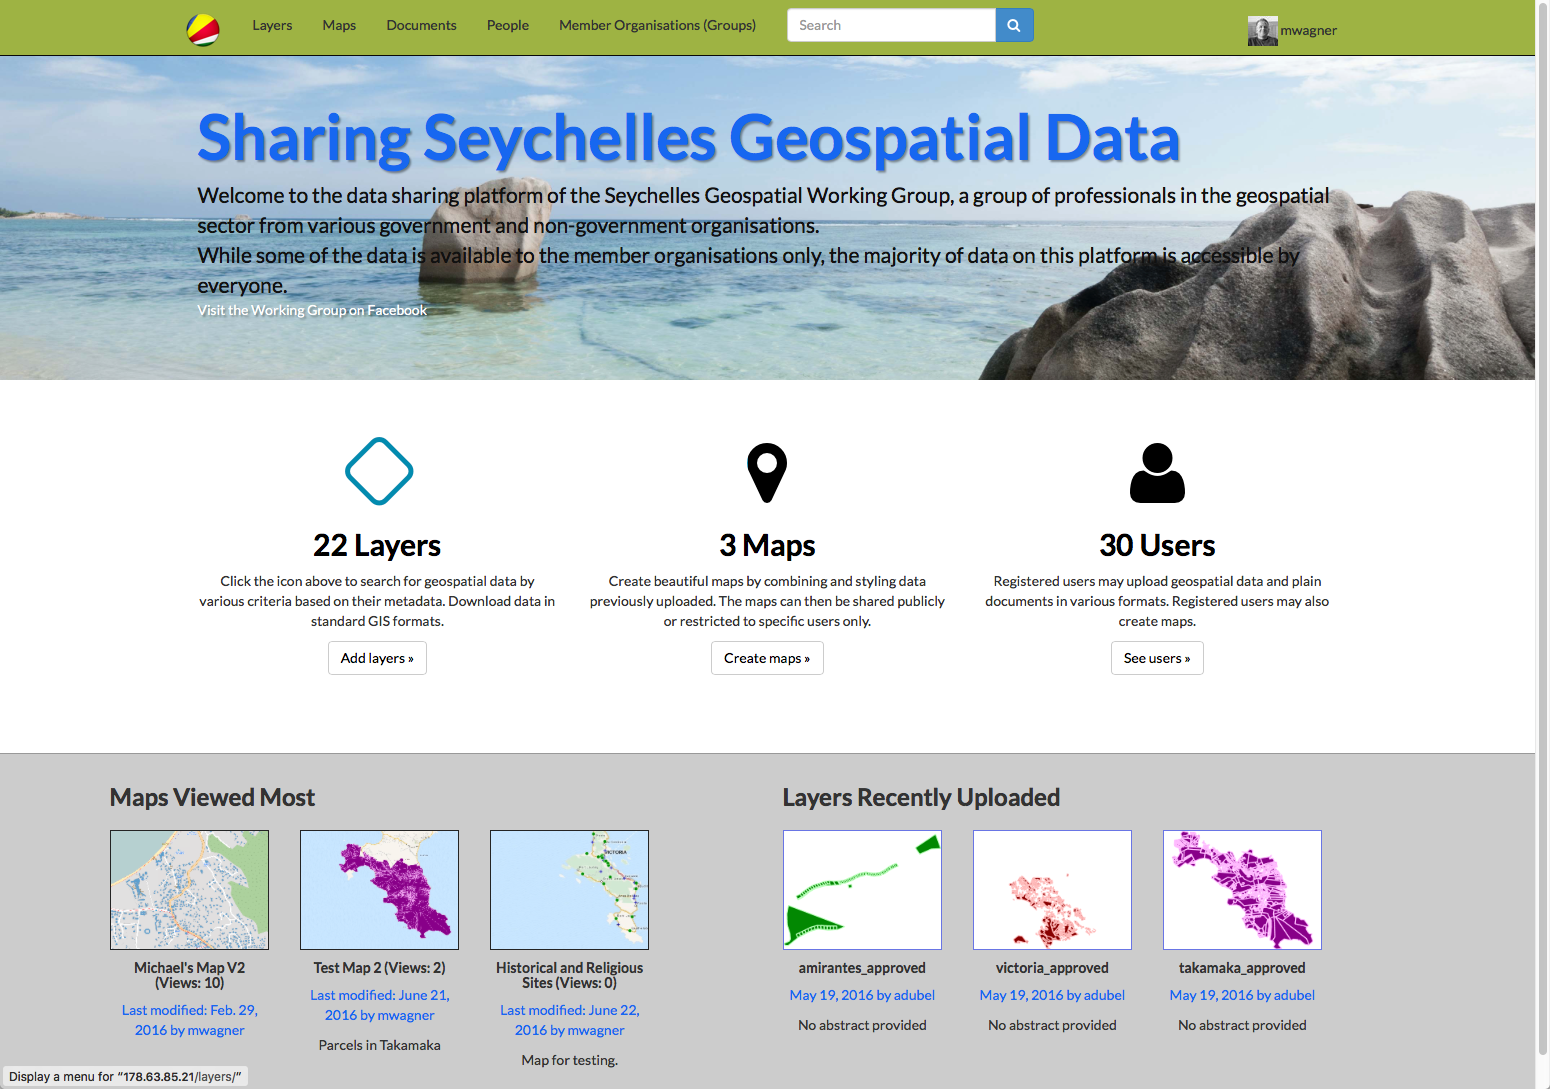
\includegraphics[width=12cm]{Images/geonode_1.png}
 	\caption{GeoNode welcome screen}\label{fig:geonode_1}
 \end{figure}
 
\subsection{First steps}

A user account has already been created for you, your username is the first letter of your first name followed by your surname (e.g. \textit{mwagner} for Michael Wagner). Your default password is \textit{XXXXXX}. You are already member of a group named after you organisation. After signing in you should first change your password and set a profile picture (Figure \ref{fig:geonode_2}). Provide also some information about yourself (such as position in your organisation , email address, etc.).

\begin{figure}[H]
\centering
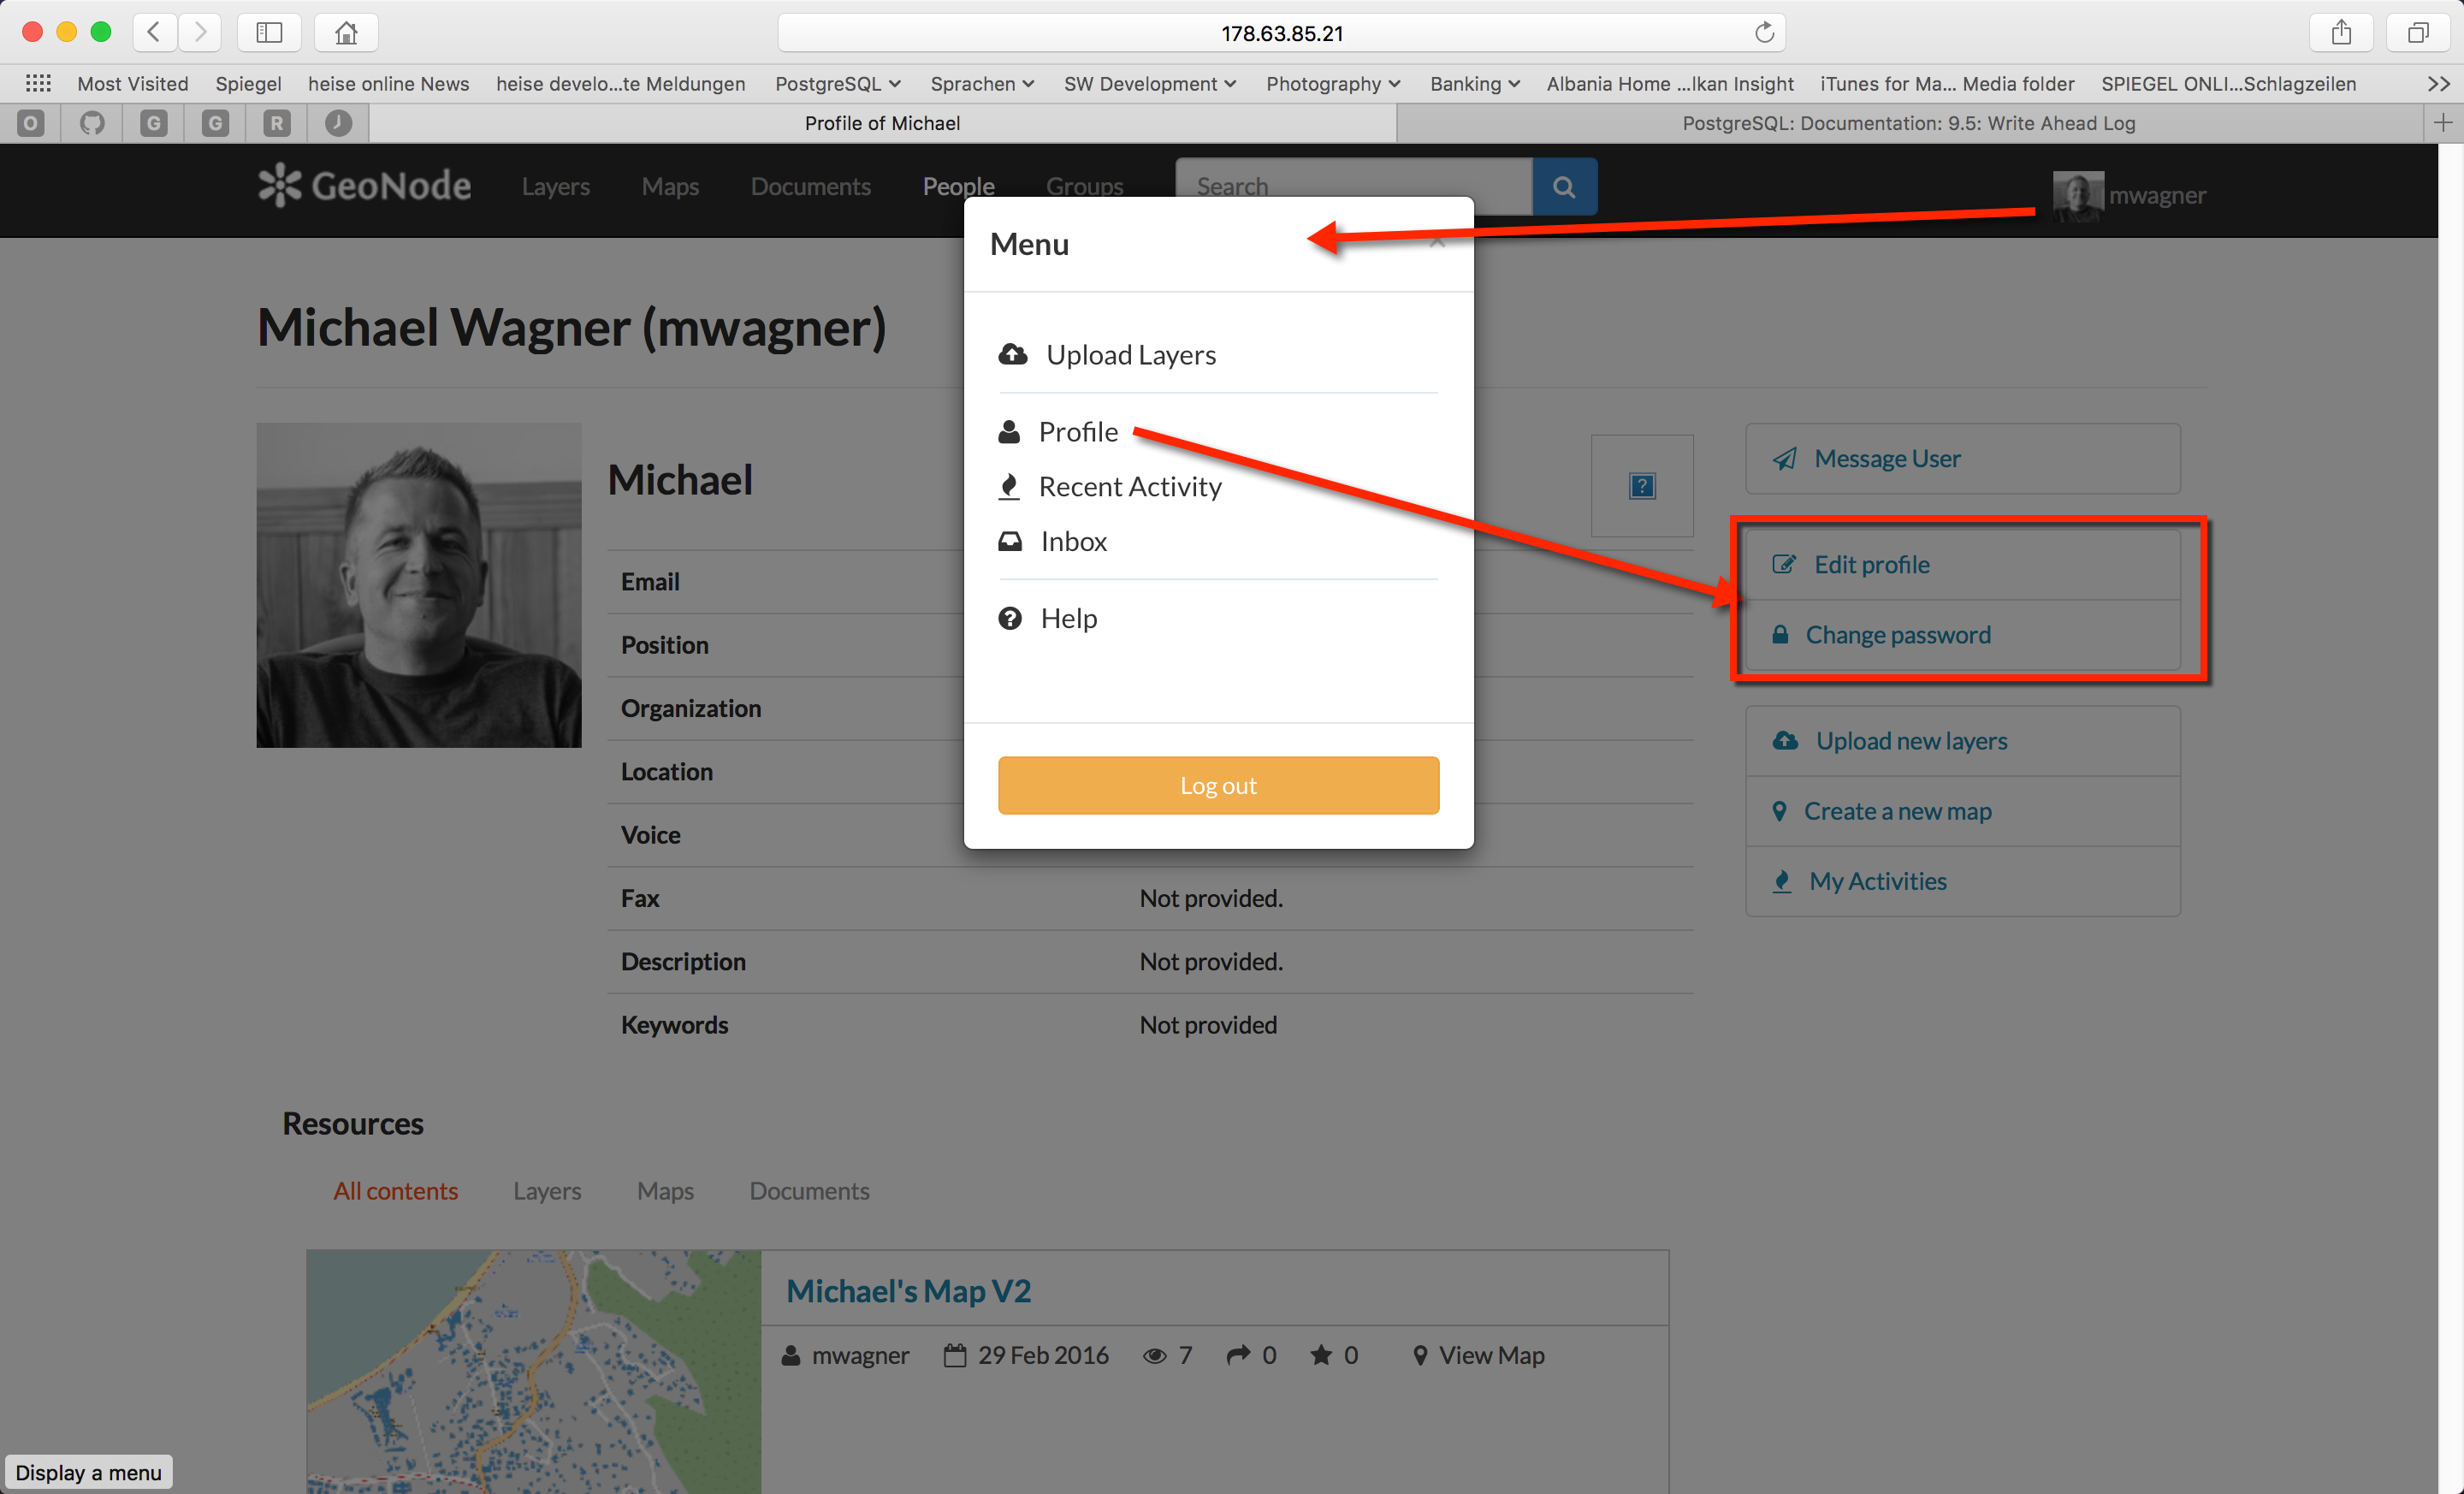
\includegraphics[width=12cm]{Images/geonode_2.png}
\caption{Changing your password and profile settings}\label{fig:geonode_2}
\end{figure}

\section{Layers}

\subsection{Uploading layers and metadata}

Once you signed in click on \textit{Layers} on the GeoNode welcome screen. You will see a list of all available layers (according to your permissions and those granted on layers by other users). Click on \textit{Upload Layers} in the upper right corner of the screen (Figure \ref{fig:geonode_3}).

\begin{figure}[H]
	\centering
	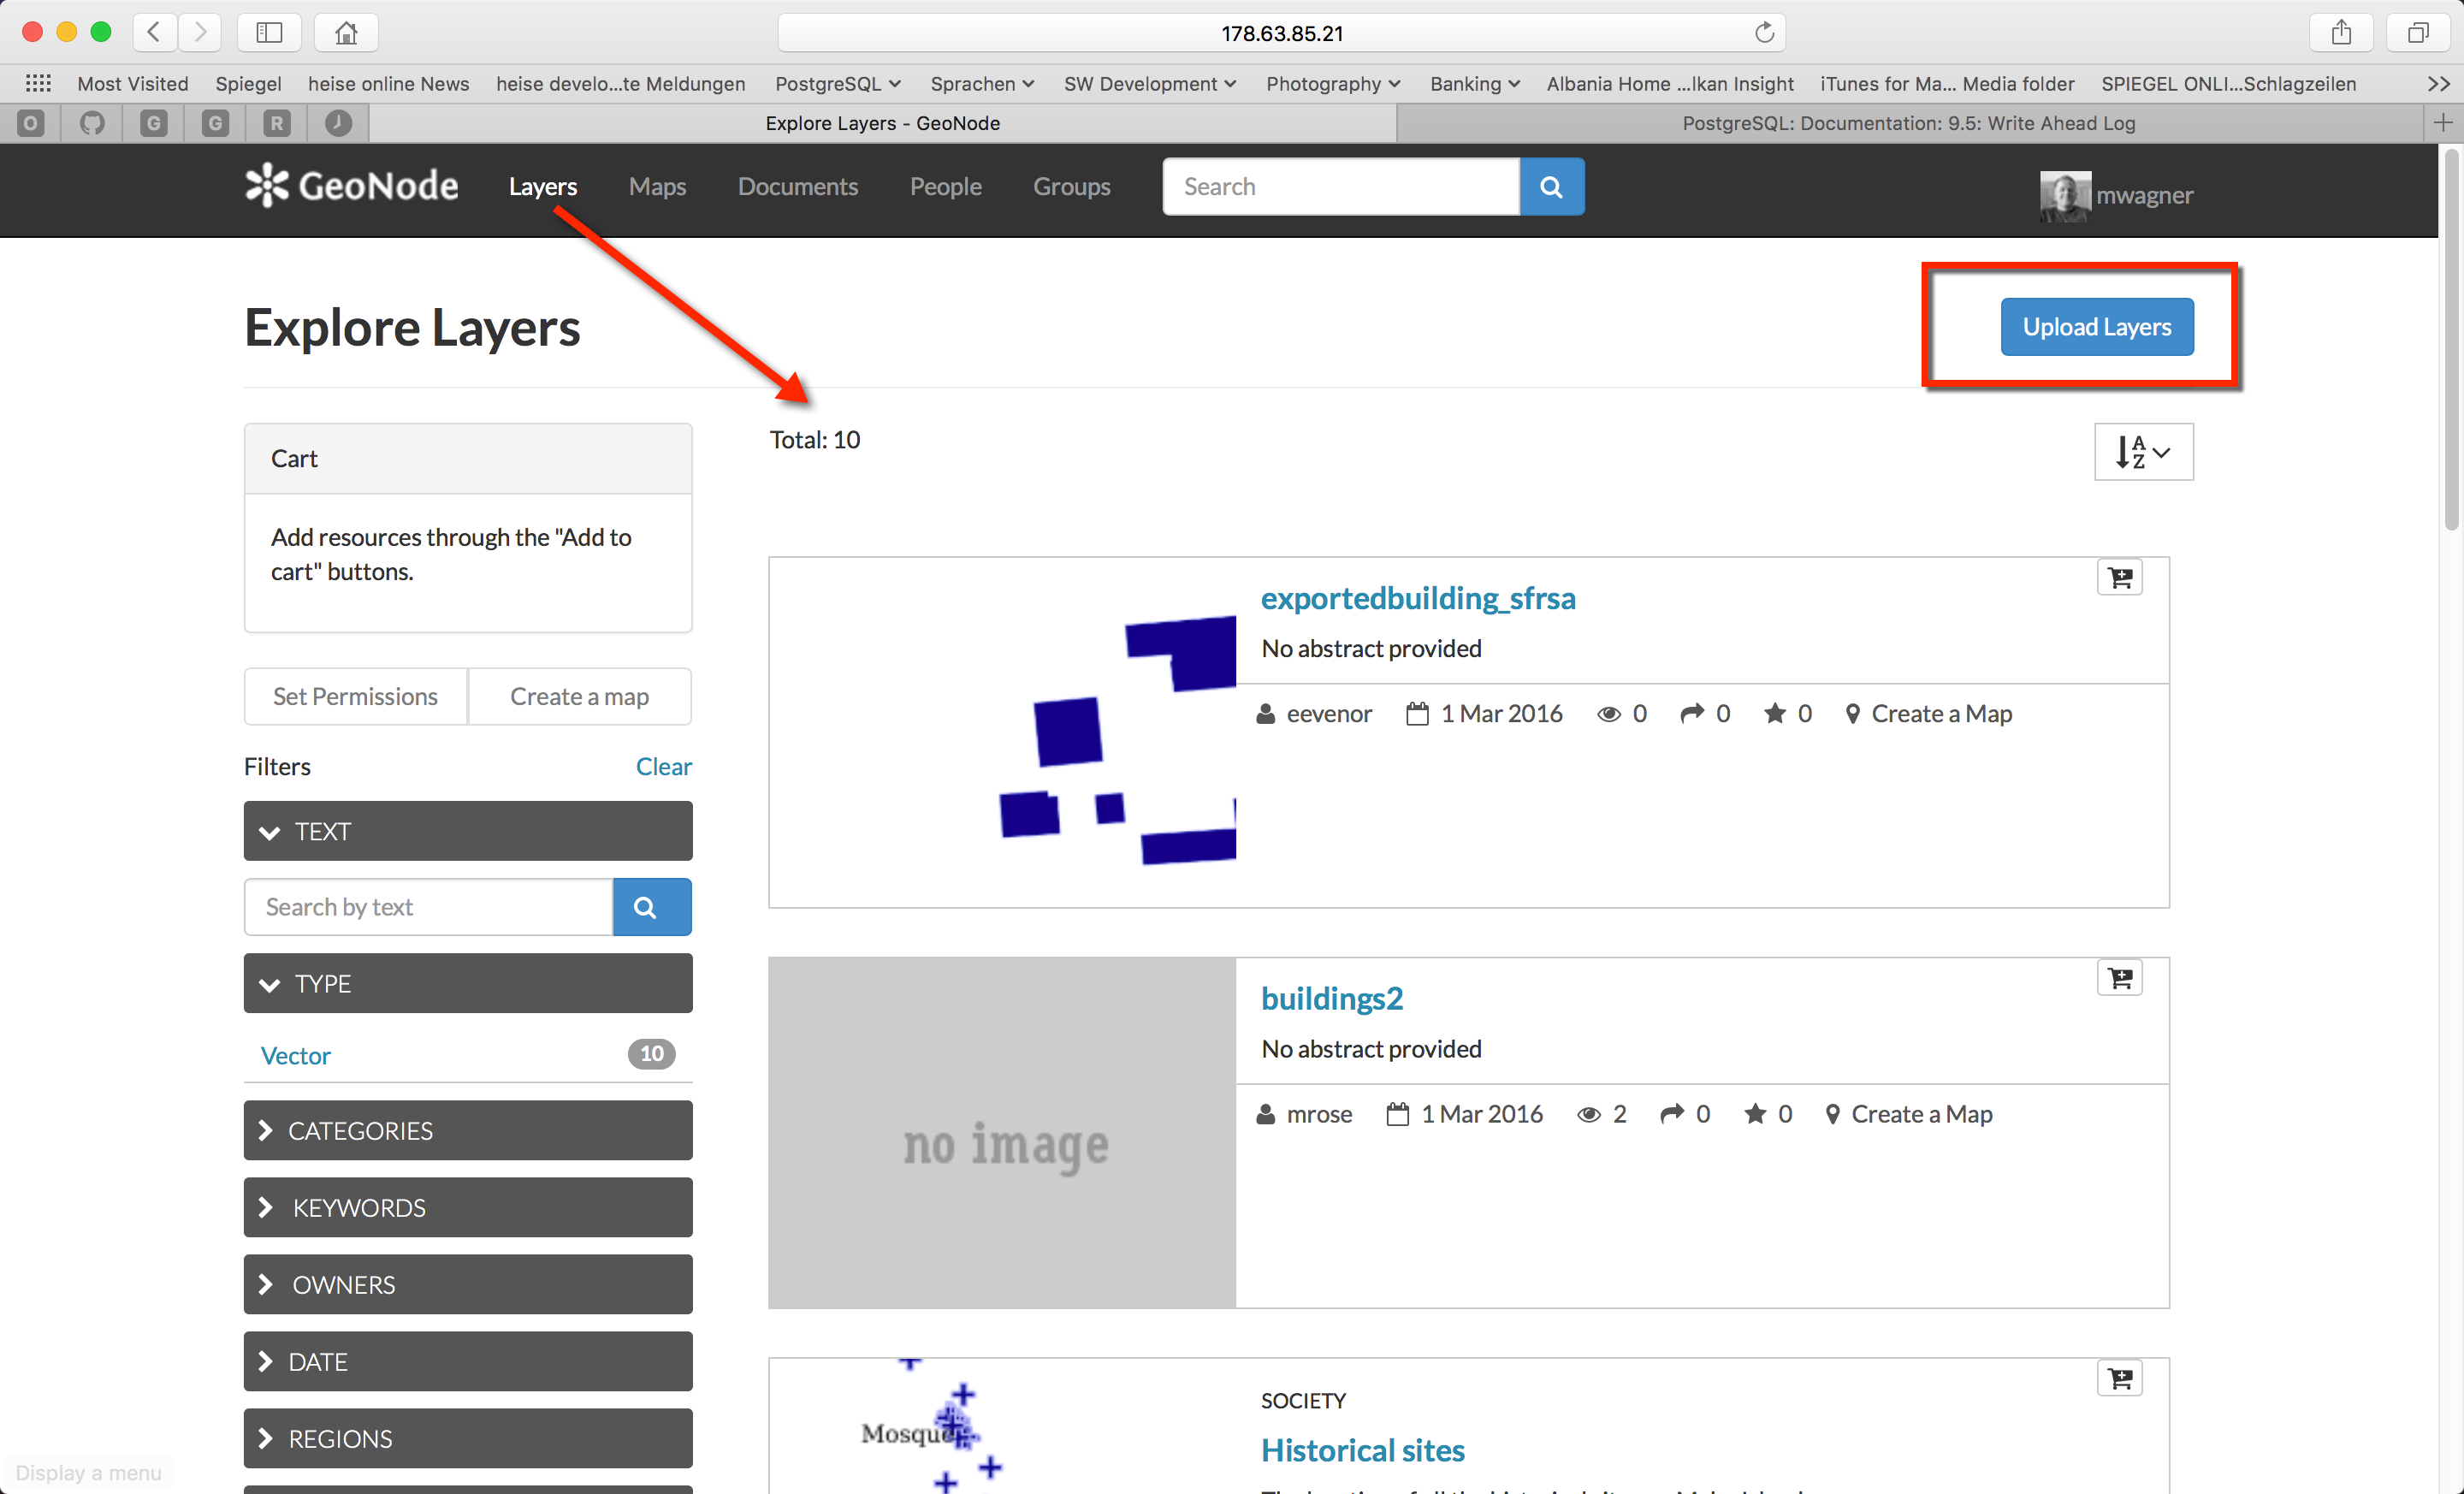
\includegraphics[width=12cm]{Images/geonode_3.png}
	\caption{GeoNode \textit{Layer} screen}\label{fig:geonode_3}
\end{figure}

Drag and drop your Shapefile and the relating metadata file to the grey area. Be aware that a Shapefile actually consists of four individual files (*.shp, *.shx, *.prj, *.dbf) and that you have to provide all of them. For the metadata to be uploaded and related to the Shapefile correctly the metadata file must have the same name as the dataset but with the ending *.xml (Figure \ref{fig:geonode_4}). The xml file you can create with any metadata editor (e.g. )\textit{CatMDEdit} or \textit{ArcCatalog}) but it must be compliant to ISOs 19115/19139. There is a flaw in the current release of GeoNode (2.4) with regard to the metadata in that only very few metadata elements are actually diggested by GeoNode (i.e. the metadata processor behind it). When you try to download metadata later on you will see that most of your original metadata elements will be missing from the file or will be empty. This is a known issue and is supposed to be fixed in the next release of GeoNode (2.5). On the right side of the screen you can set the permissions on the layer. Finally click the \textit{Upload files} button.

\begin{figure}[H]
	\centering
	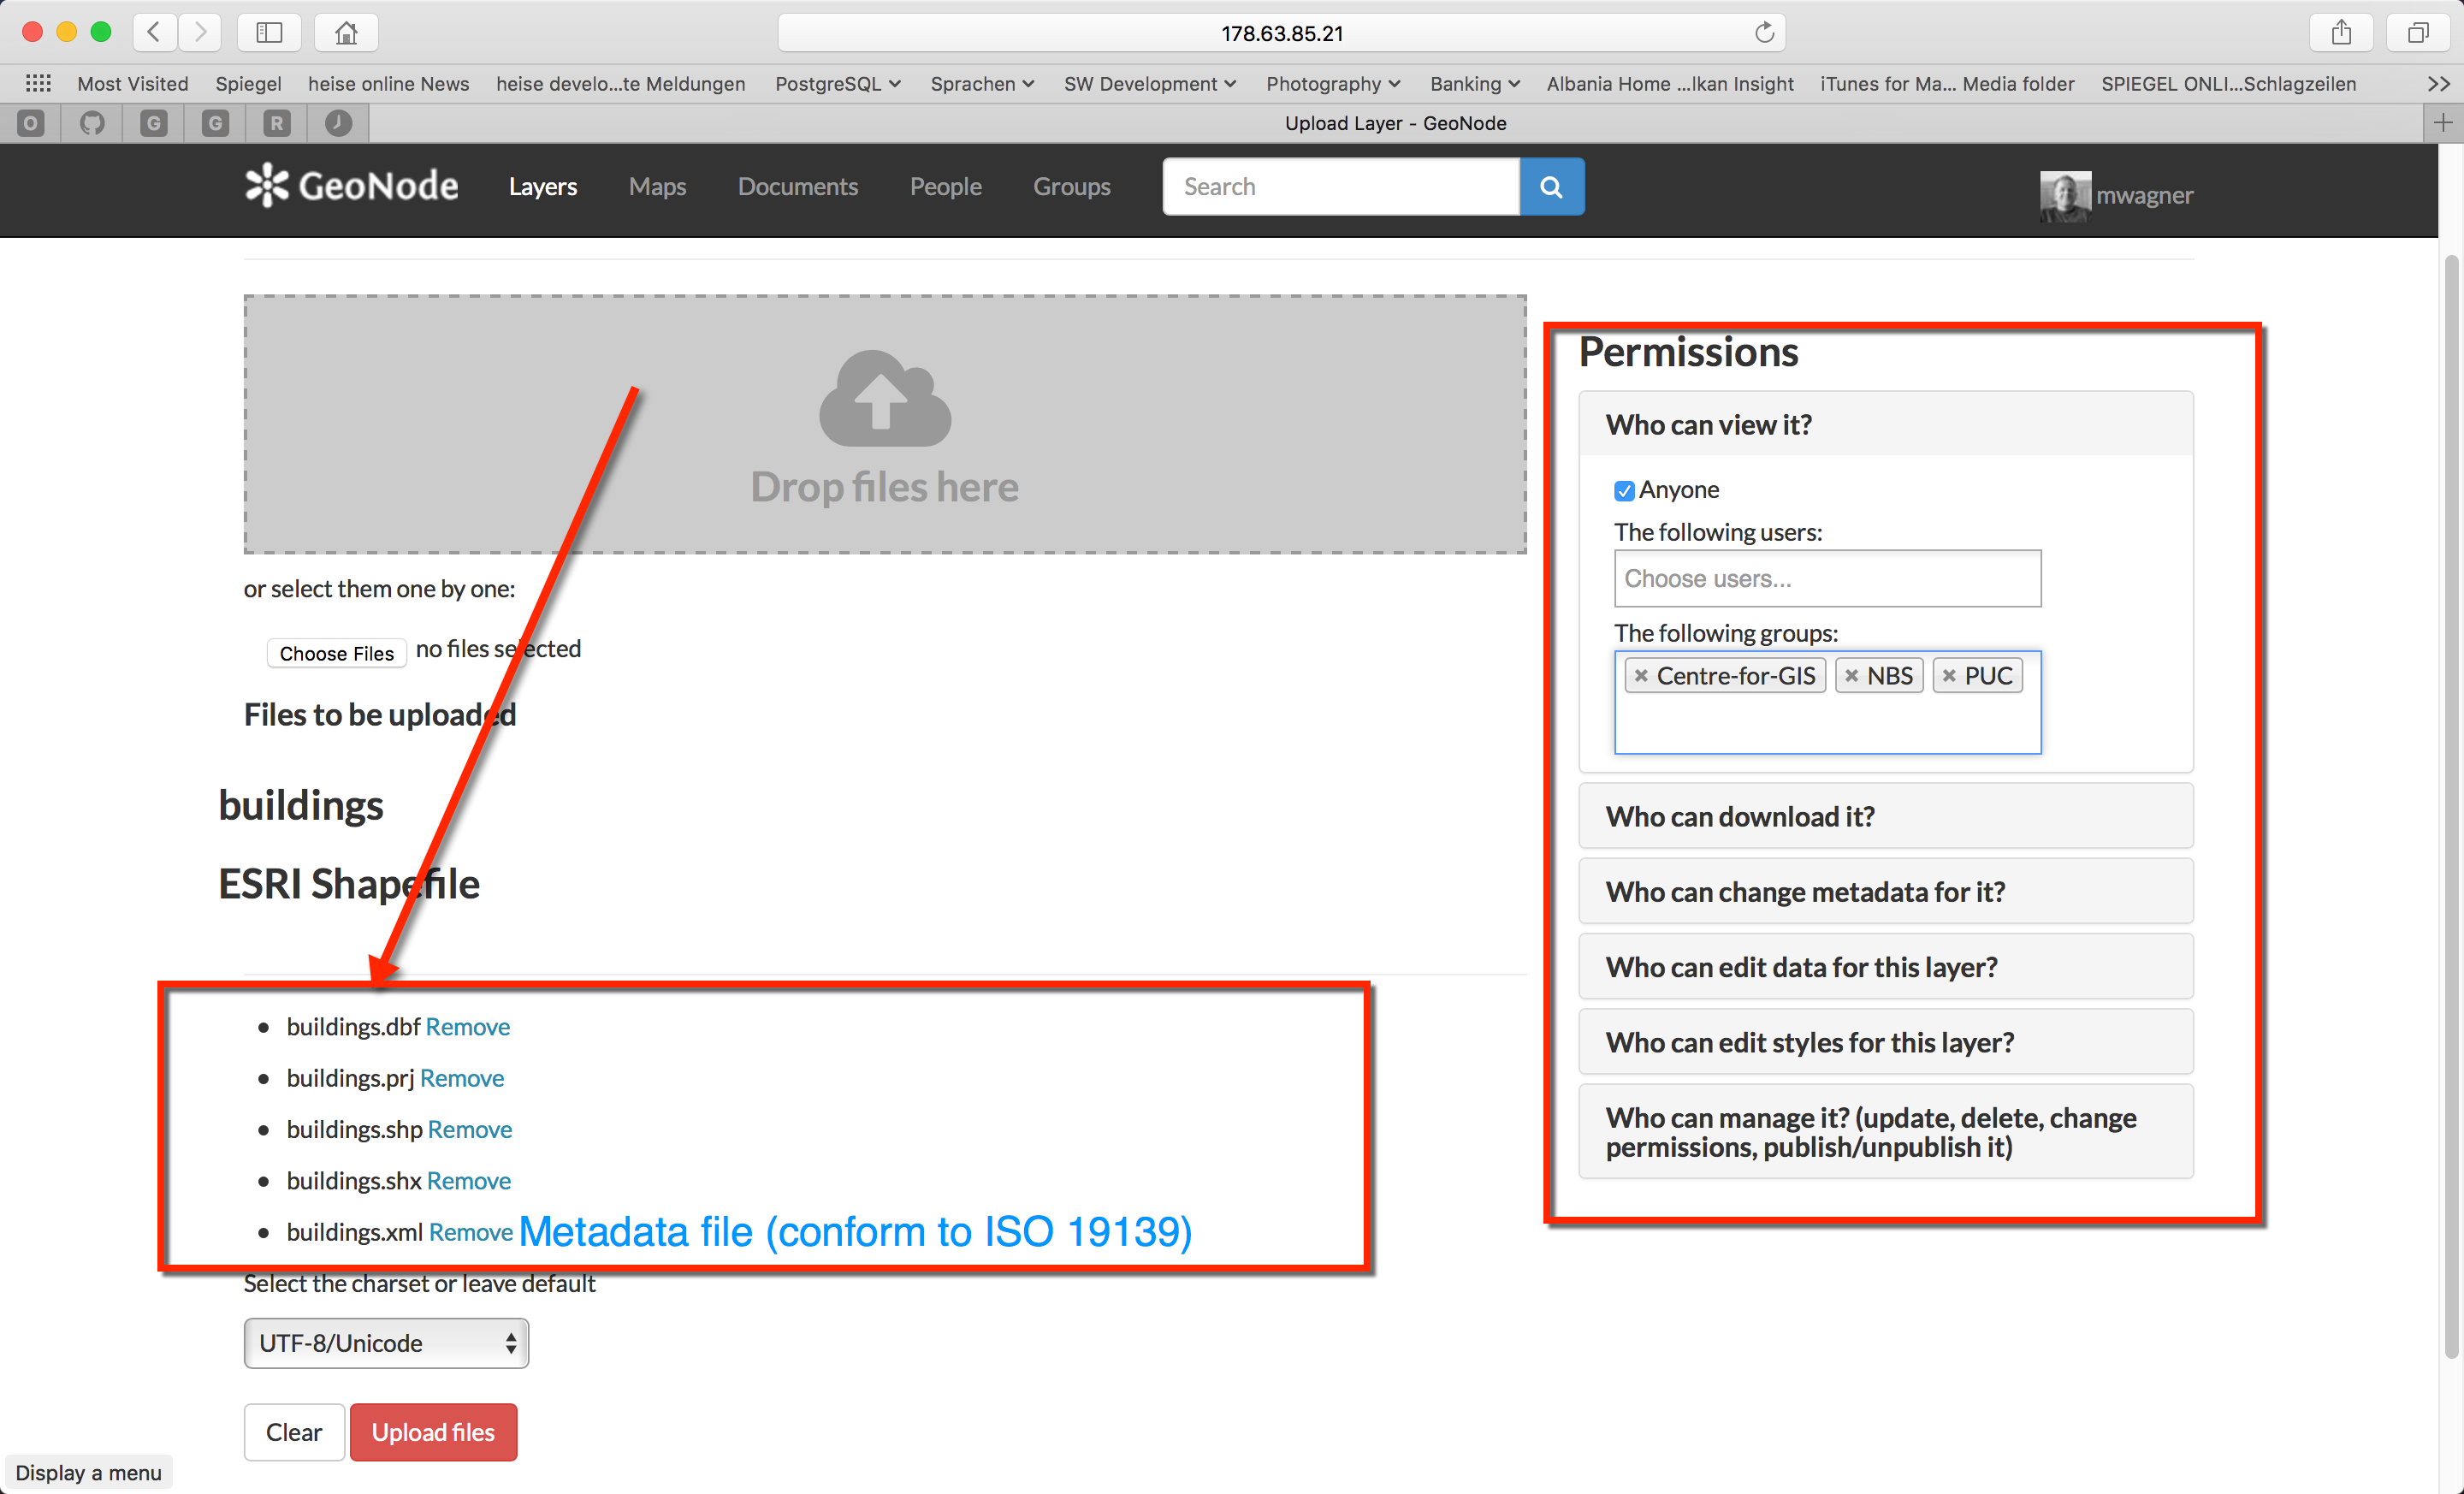
\includegraphics[width=12cm]{Images/geonode_4.png}
	\caption{Uploading a layer}\label{fig:geonode_4}
\end{figure}

Once the upload has finished your layer should be listed under the \textit{Layers} category/menu.
Following this workflow you should upload all your disaster relevant datasets (according to the dataset list available at \textit{Trello}).
For the time being it is recommended that you upload your vector datasets only. Once the GeoNode server is accessible through the government network you can (and should) also upload your raster data. Otherwise the raster data might eat up yours or your organisation's Internet data package.

\subsection{Setting permissions}

As mentioned in the previous section permissions for a layer can be set during the upload of the dataset but also afterwards. Under the aspect of data sharing by default anyone can see and download the layer you uploaded (i.e. without setting any permissions explicitly). However, that might not be acceptable for your organisation. Thus, you can set permissions for individual users or for a group (Figure \ref{fig:permissions}). If set for a group -- any user who is member of that group will have access to the layer. By default only the owner of a layer can change permissions. If the \textit{View} permission is not granted the layer will not be shown in the list of layers.

\begin{figure}[H]
	\centering
	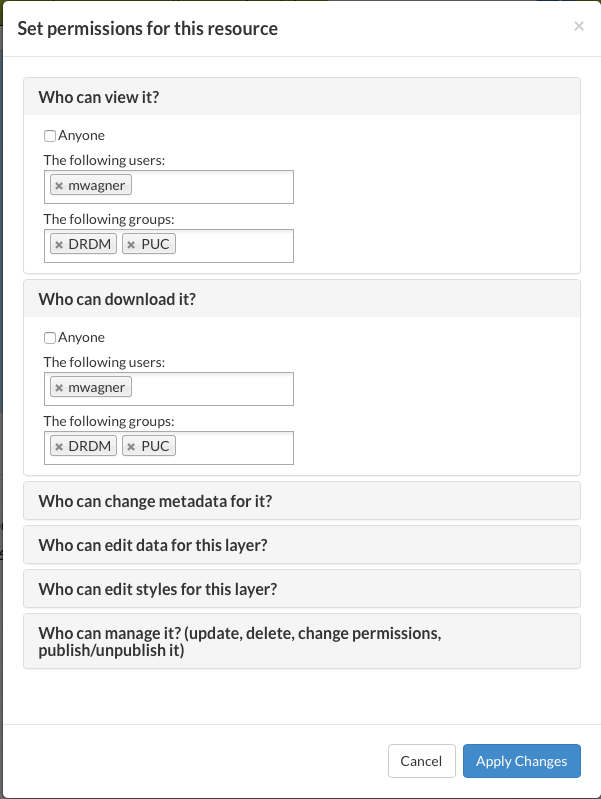
\includegraphics[width=8cm]{Images/permissions.png}
	\caption{Setting layer permissions}\label{fig:permissions}
\end{figure}

\subsection{Editing layer styles and metadata}

Styles and metadata can be edited by the layer owner and those users and/or groups who have been granted the required permission.
The \textit{Edit Layer} button will then be available through which you can access the metadata editor and style editor (Figure \ref{fig:edit_layer}). The GeoNode version currently installed has a bug with regard to the layer styles. A change made with the style editor is not reflected and opening the style editor again will show the same original style. A workaround to deal with that is to set the style directly in GeoServer.

\begin{figure}[H]
	\centering
	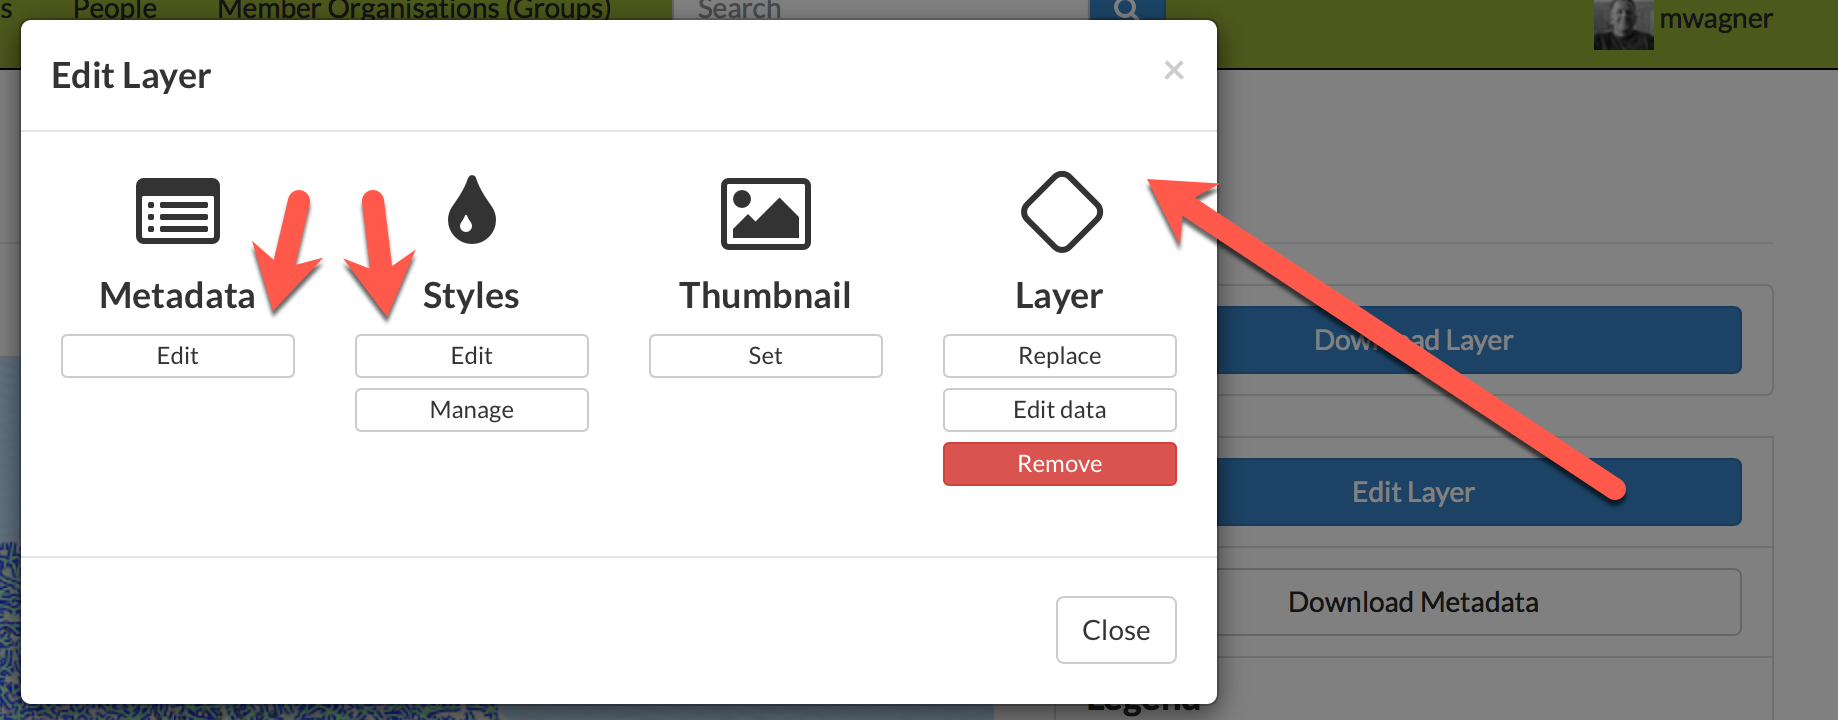
\includegraphics[width=12cm]{Images/edit_layer.png}
	\caption{Editing a layer's style or metadata}\label{fig:edit_layer}
\end{figure}

\subsection{Downloading layers and metadata}

Layers can be downloaded in various GIS formats (Figure \ref{fig:supported_formats}). For the relating metadata the most common metadata standards are supported (e.g. ISO 19115/19119, Dublin Core, etc.). 

\begin{figure}[H]
	\centering
	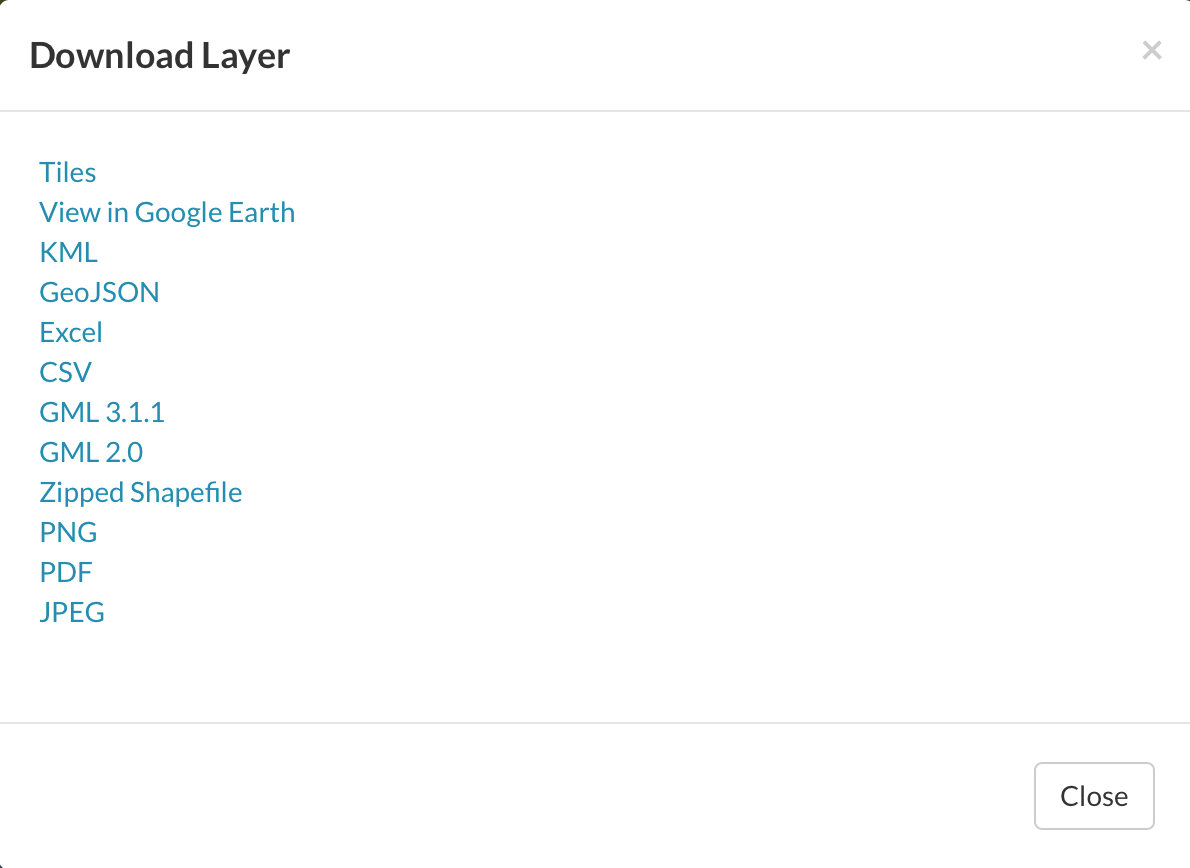
\includegraphics[width=8cm]{Images/supported_formats.png}
	\caption{Supported download formats for vector data}\label{fig:supported_formats}
\end{figure}

\section{Documents}

\subsection{Uploading documents}

Any non-spatial datasets can be uploaded through the \textit{Documents} section.
You can select a single file to be uploaded, set the relating permissions and click the \textit{Upload} button. If a document should be linked to an existing layer or map this can be set before the upload (Figure \ref*{fig:geonode_5}) or afterwards by editing the document's metadata.
 
\begin{figure}[H]
	\centering
	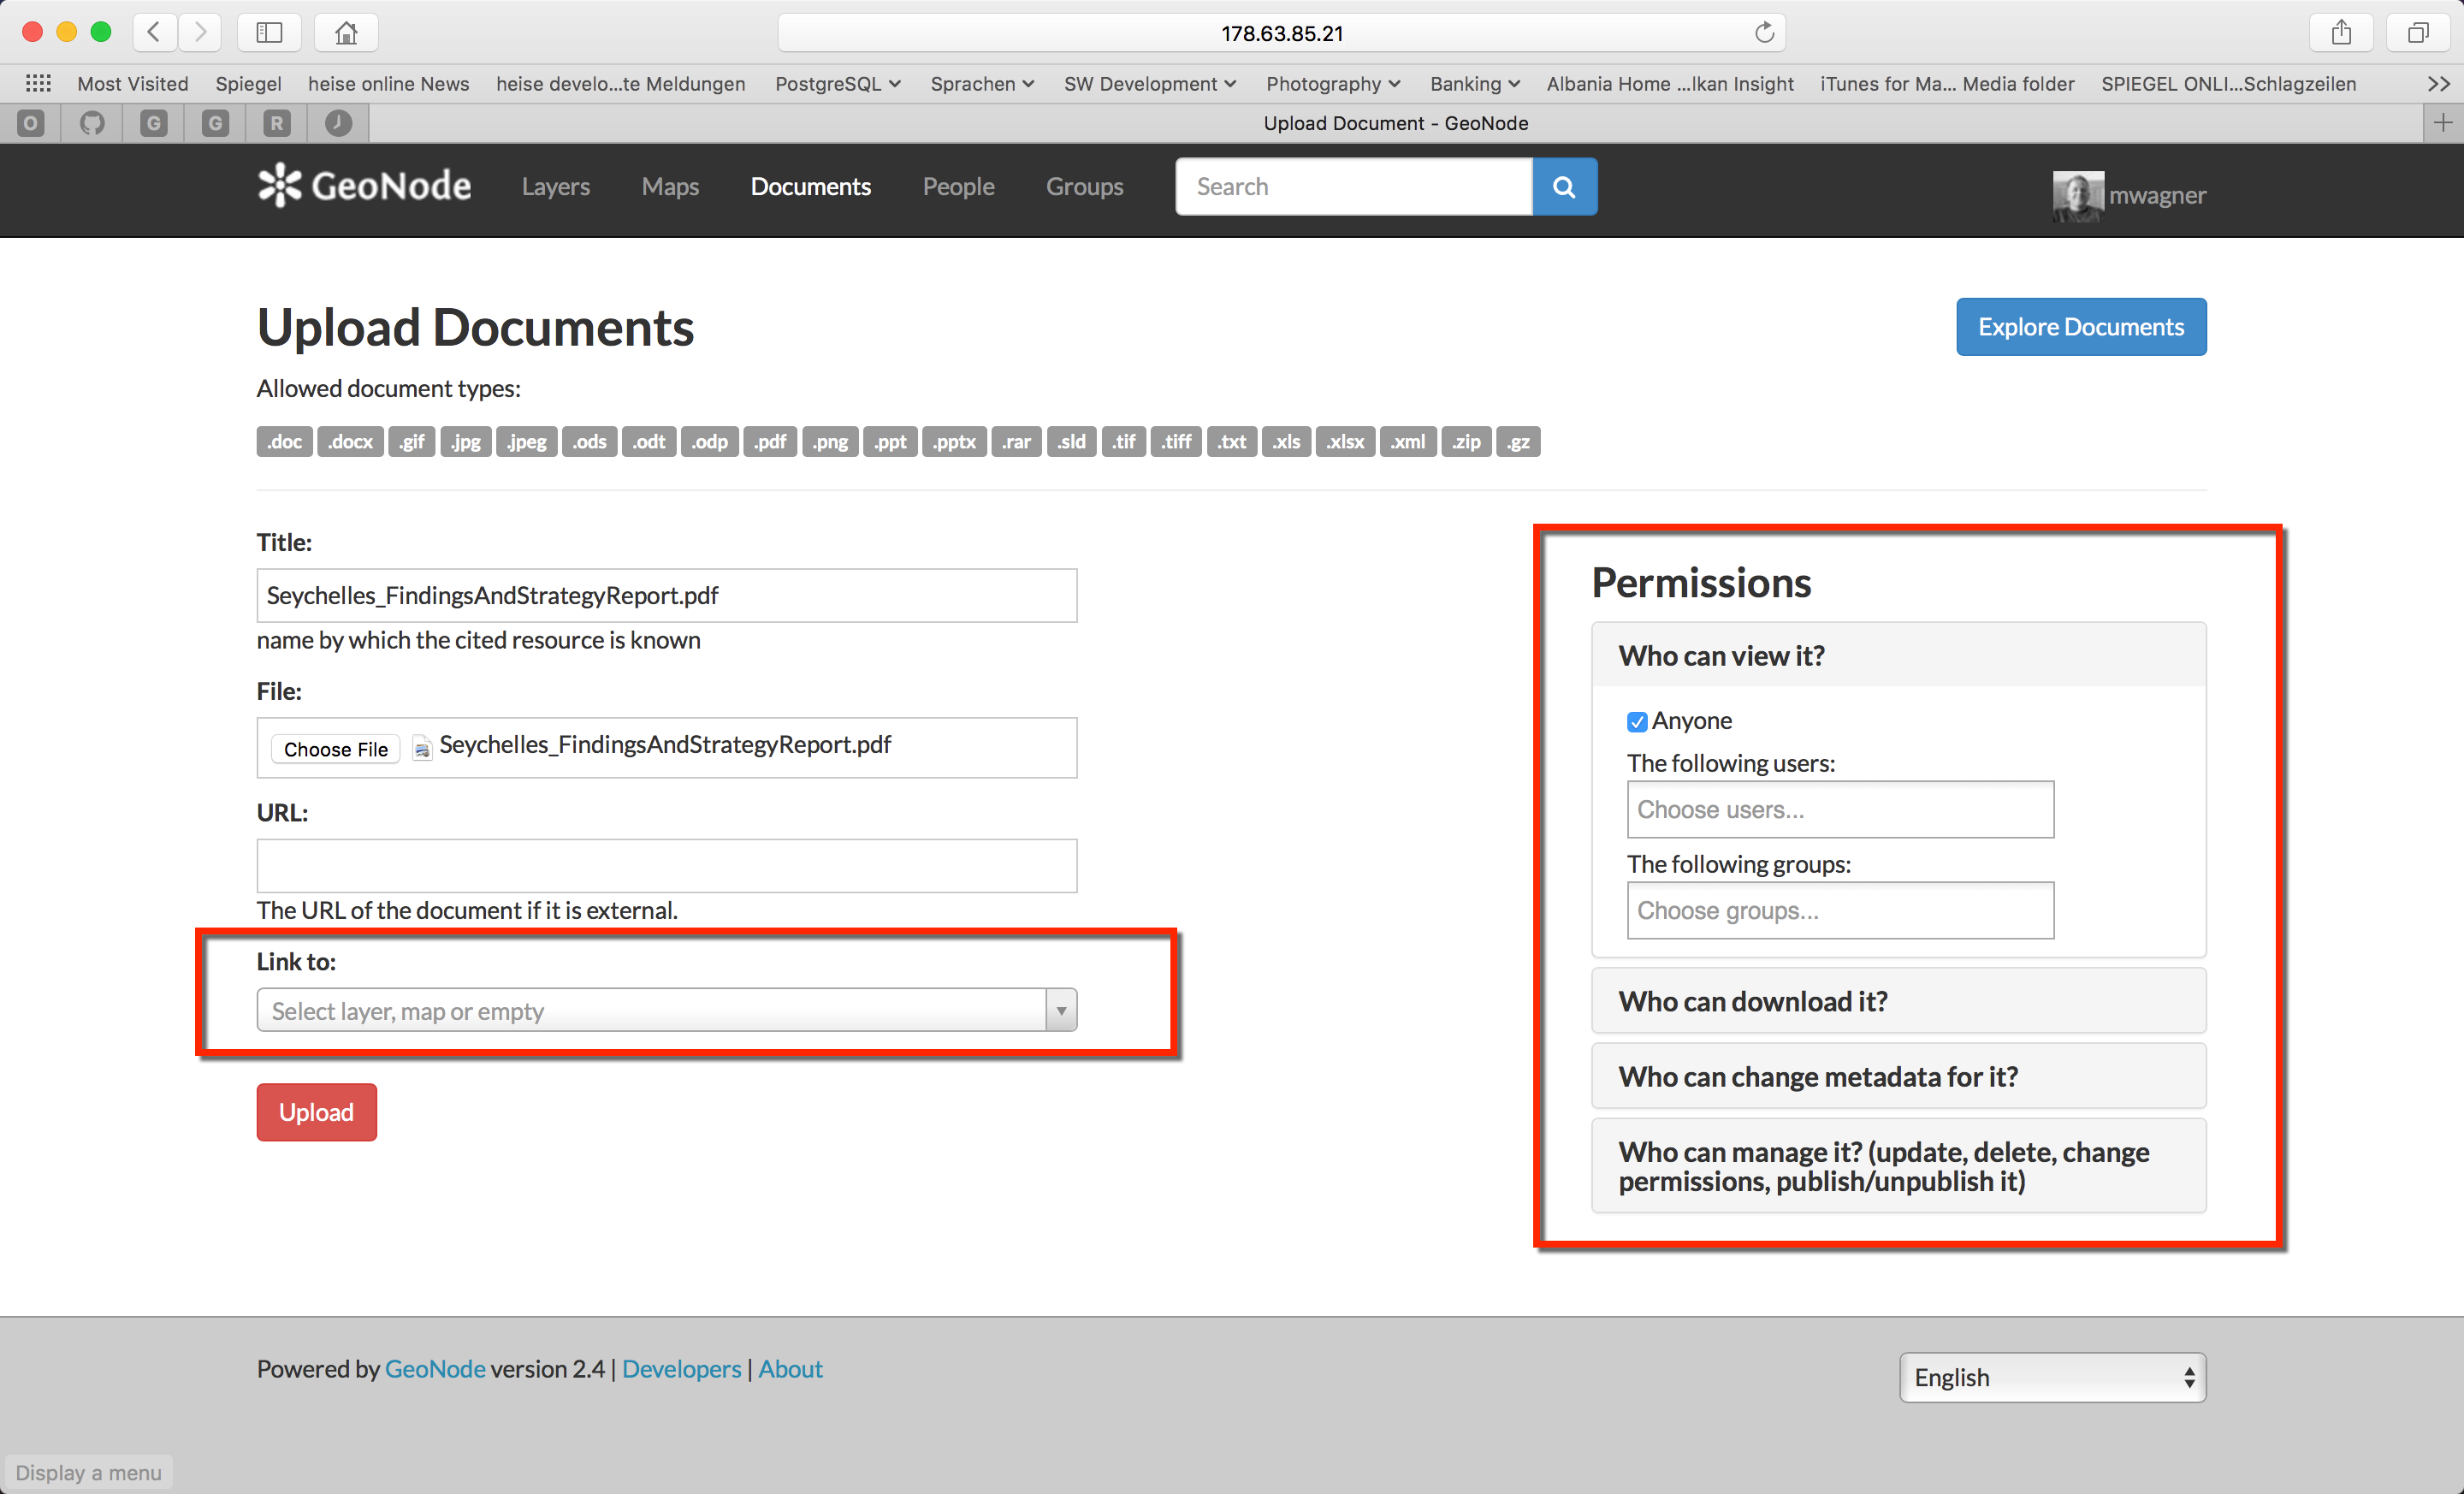
\includegraphics[width=12cm]{Images/geonode_5.png}
	\caption{Uploading a document}\label{fig:geonode_5}
\end{figure}

\subsection{Setting permissions}

Permissions can be set during the document upload or afterwards. If the \textit{View} permission is not granted the document will not be shown in the list of documents.

\subsection{Editing document metadata}

\textit{Editing} a document means actually editing its metadata or simply deleting the document. A number of metadata elements can be set for a document such as title, abstract, keywords, etc.

\subsection{Downloading documents}

Not much to explain here. Downloading a document is straightforward.

\section{Maps}

\subsection{Creating and editing maps}

Maps can be created by combining/overlaying layers previously uploaded. GeoNode also provides a number of base maps from OpenStreetMap (Figure \ref{fig:map1}). Additional base maps (e.g. Google or Bing) can be added by a GeoNode administrator but require to obtain an API key from the map/service provider (e.g. Google or Microsoft). Furthermore users can add layers from a Web Map Service (WMS) (Figure \ref{fig:map2}). Maps can be created by anyone but be saved by registered users only.

\begin{figure}[H]
	\centering
	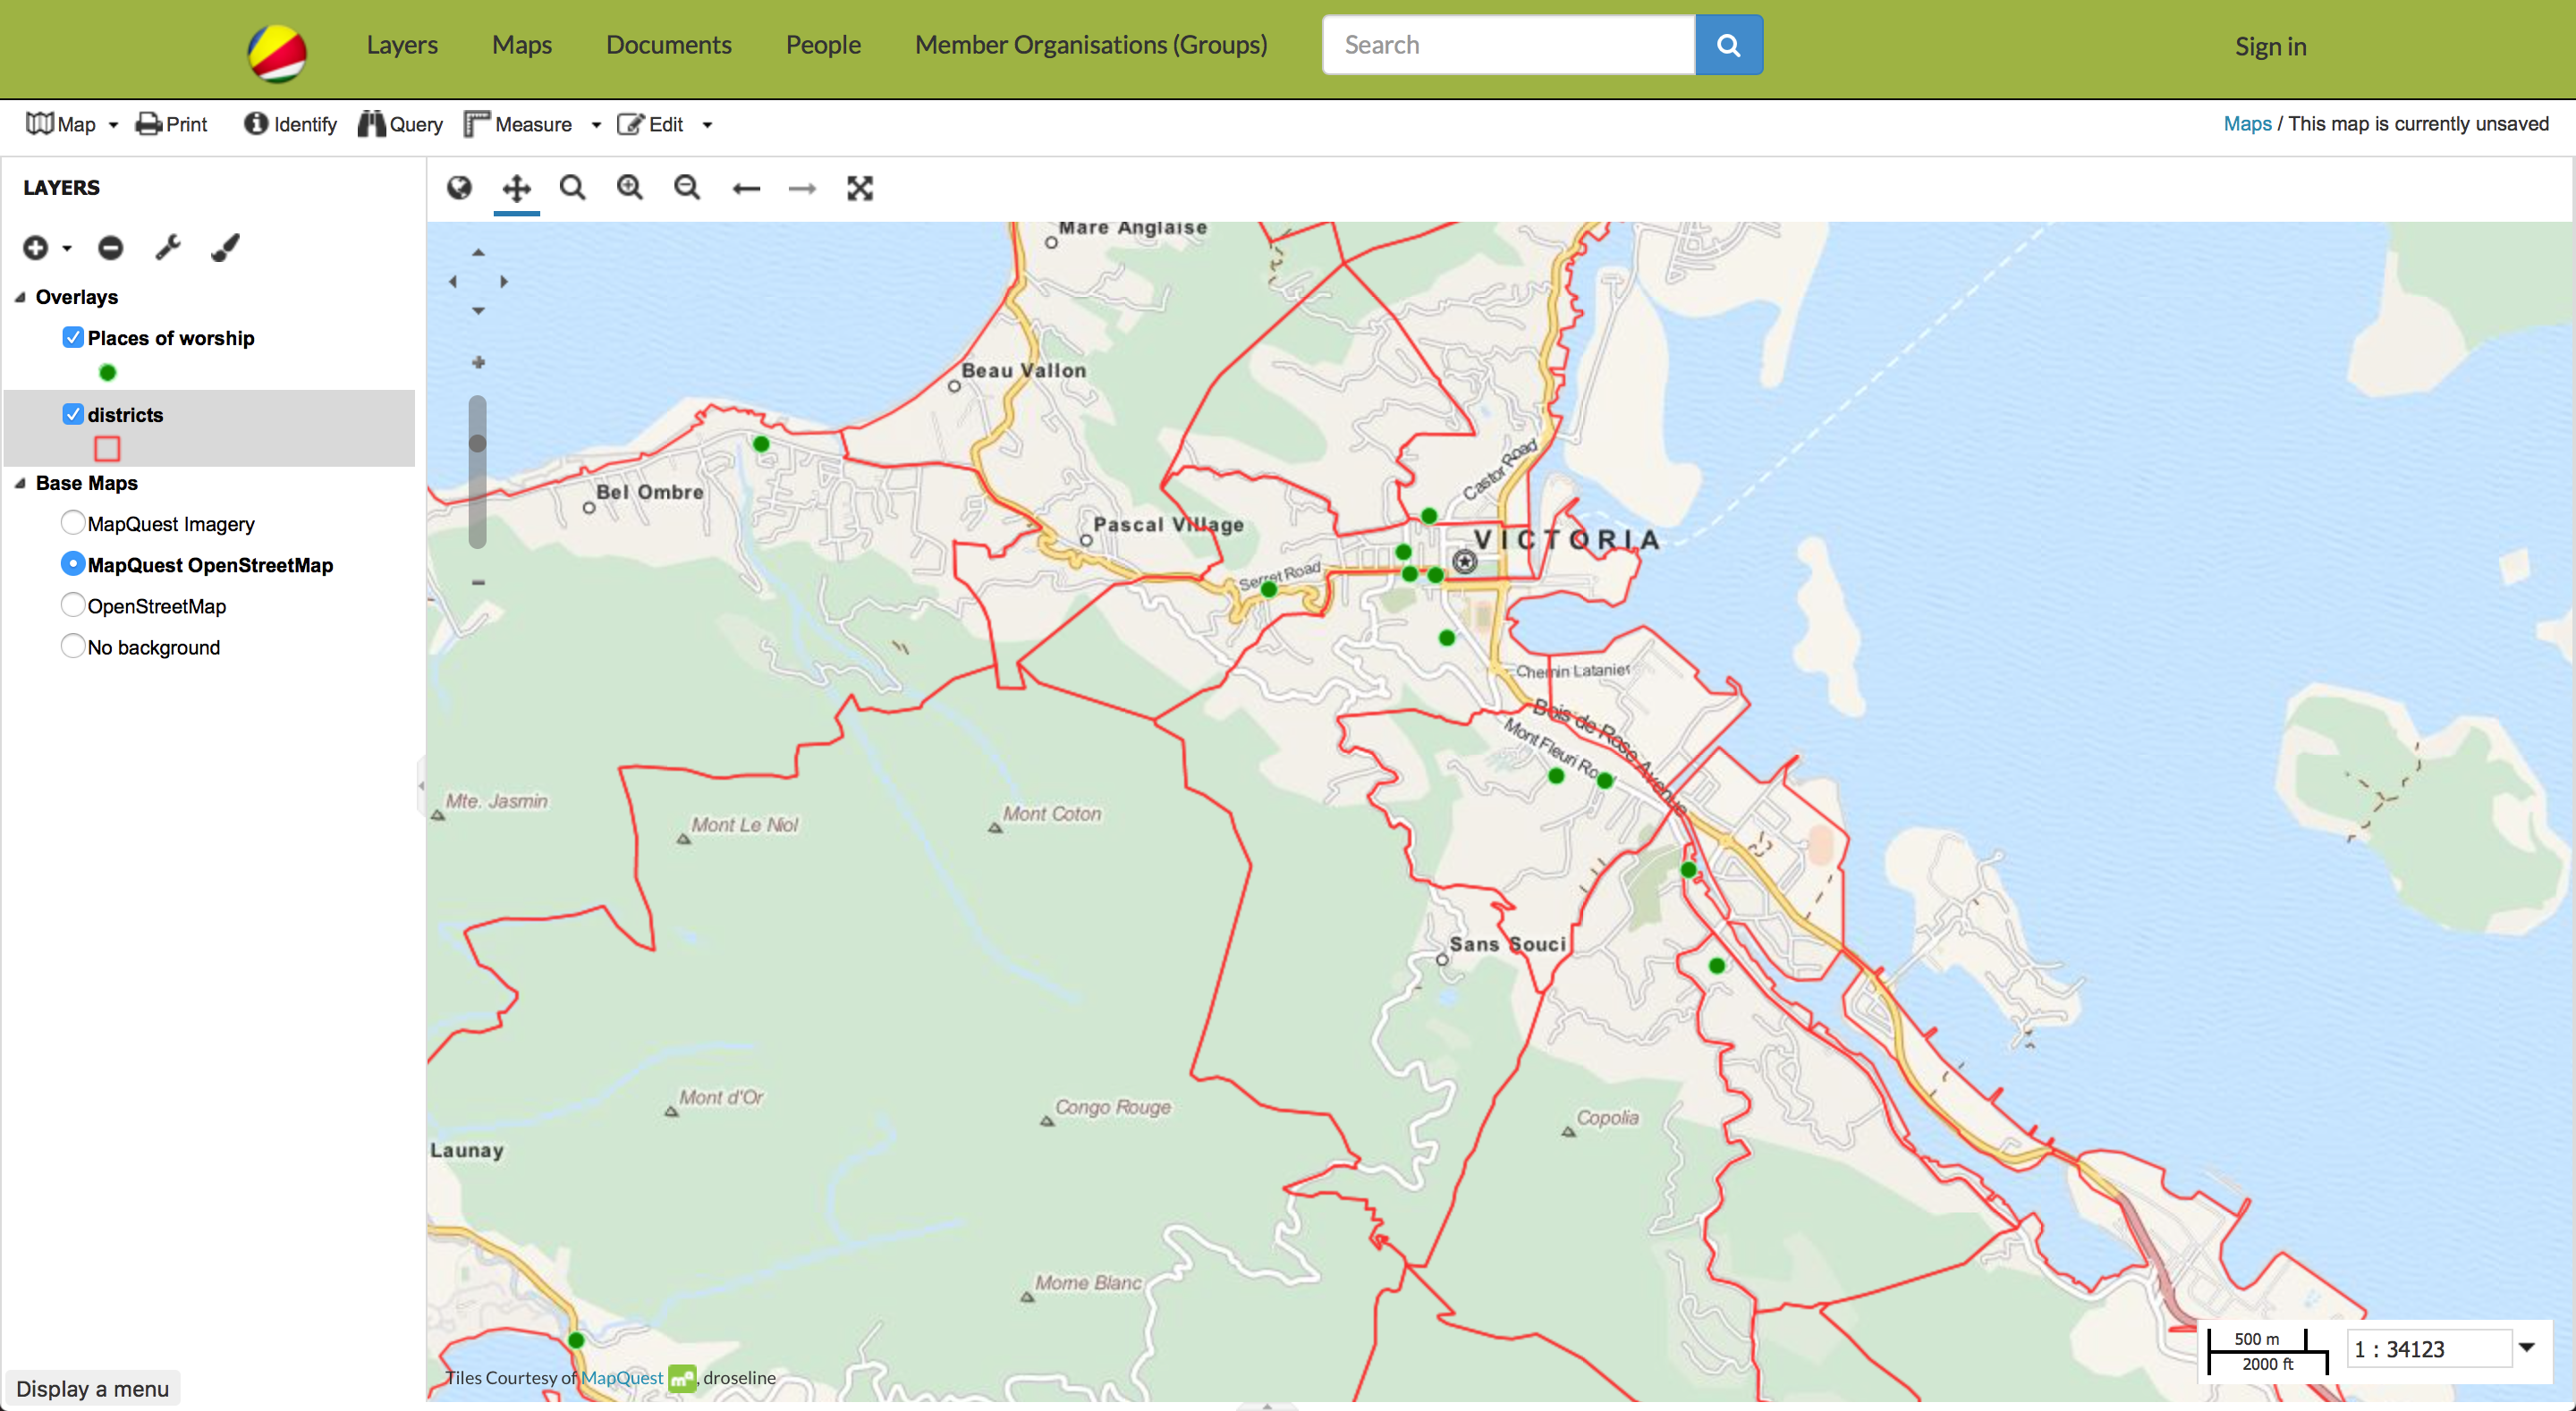
\includegraphics[width=12cm]{Images/map1.png}
	\caption{Creating a map in GeoNode}\label{fig:map1}
\end{figure}

\begin{figure}[H]
	\centering
	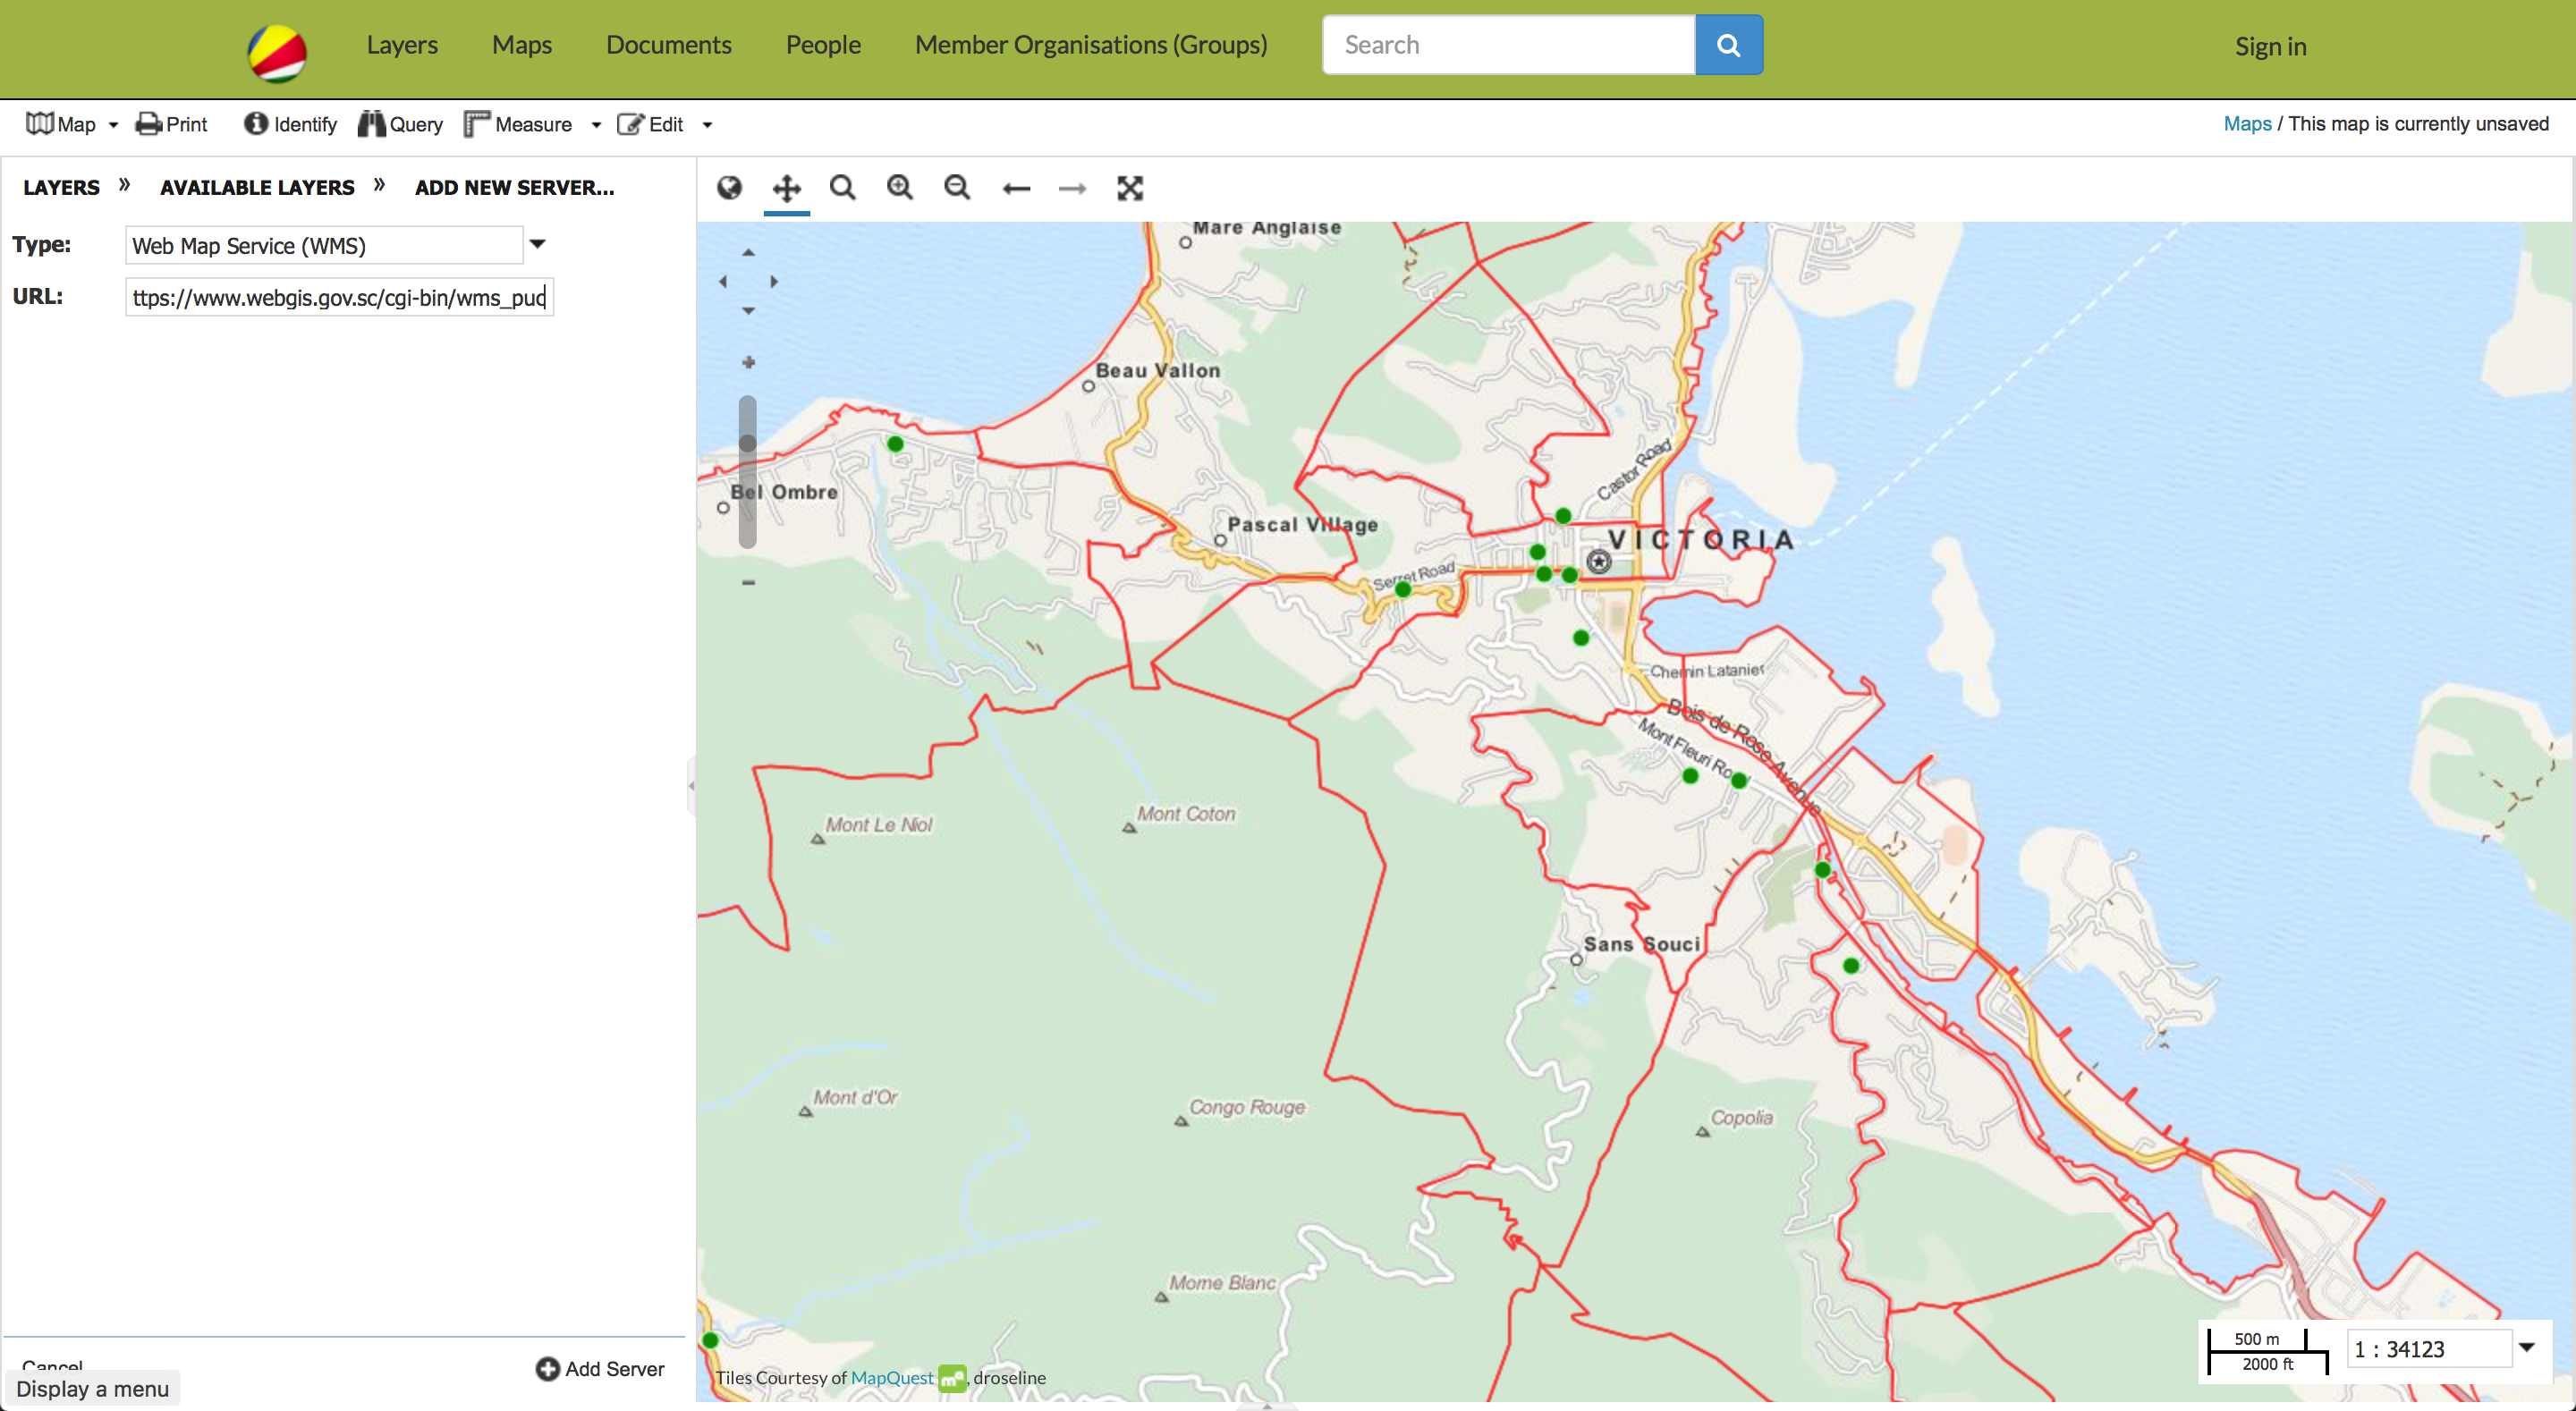
\includegraphics[width=12cm]{Images/map2.png}
	\caption{Adding a Web Map Service}\label{fig:map2}
\end{figure}

\subsection{Setting map permissions}

Permissions can be set with regard to who can view or edit a map. Editing a map means adding or removing layers. Without a \textit{View} permission a user won't be able to see a map in the list of maps.

\subsection{Editing map metadata}

A number of metadata elements can be set for a map such as title, abstract, keywords, etc.

\subsection{Publishing maps}

A map in GeoNode can be published, i.e. an HTML code snipped is generated which can be embedded in any HTML page (e.g. the website of your organisation). A map can be published once the map is in \textit{View} mode (Figure \ref{fig:map3}).

\begin{figure}[H]
	\centering
	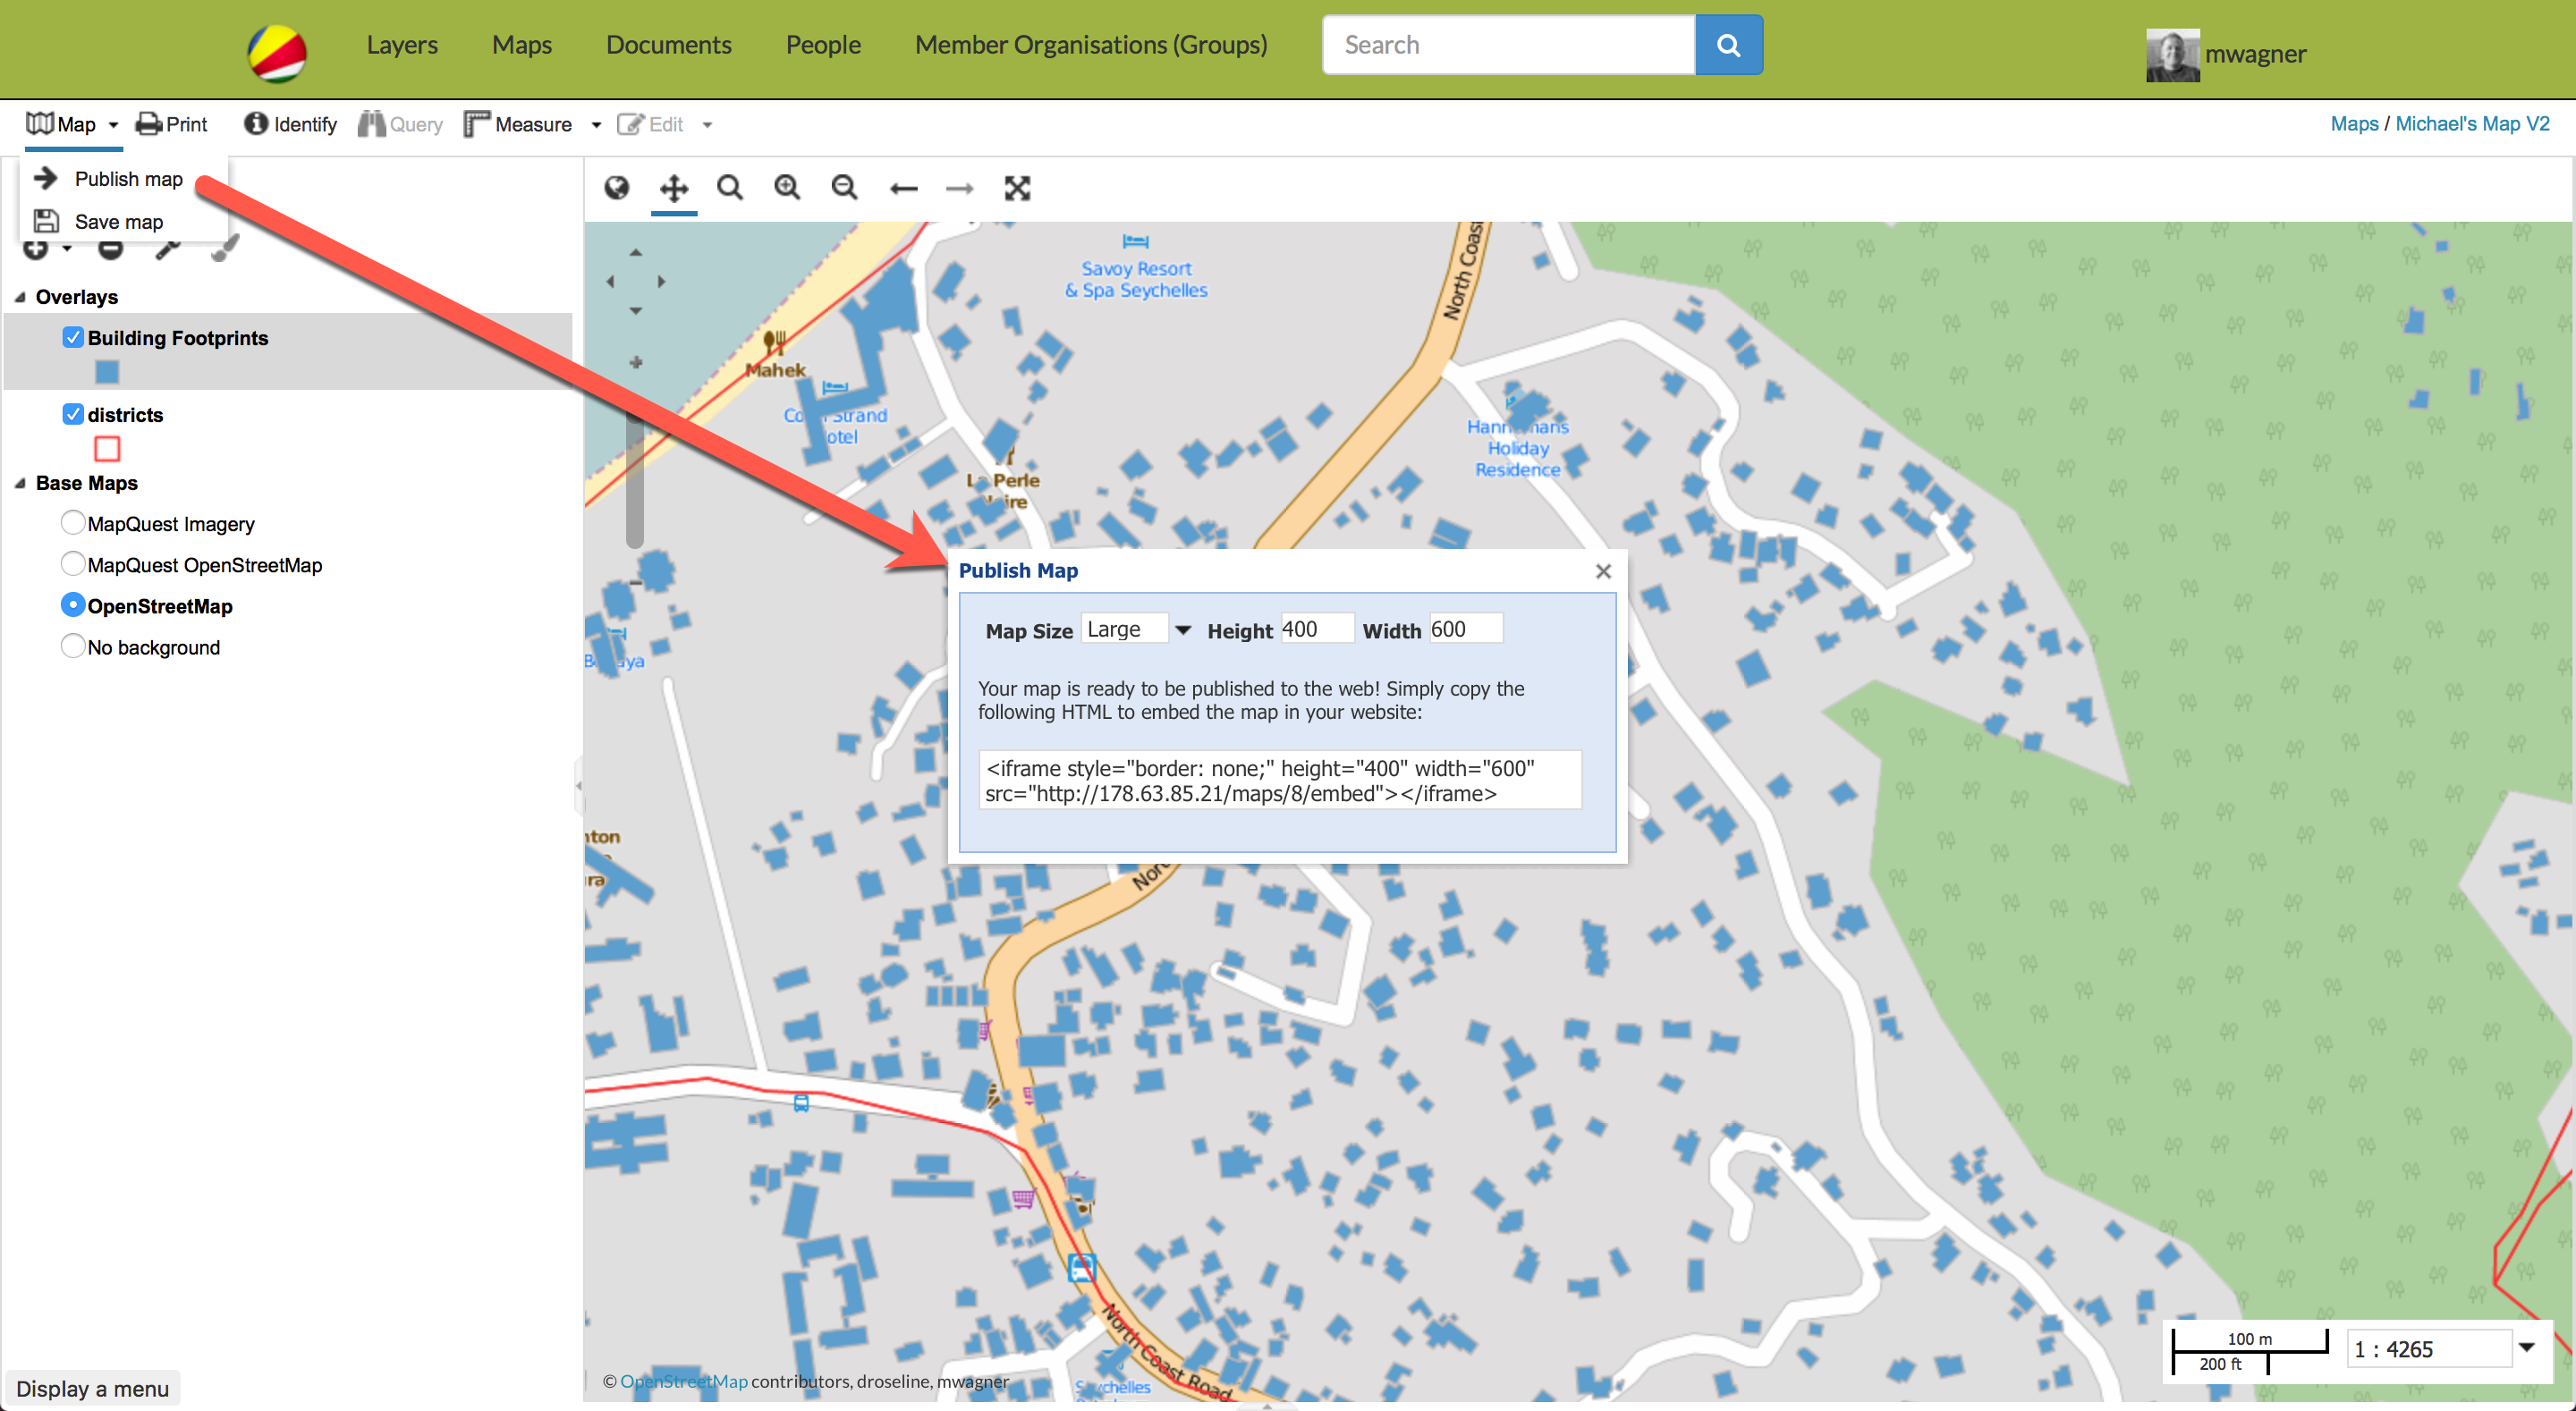
\includegraphics[width=12cm]{Images/map3.png}
	\caption{Publishing a map}\label{fig:map3}
\end{figure} 

\section{Basic administration}

To administrate GeoNode you need to have superuser privileges. Log on as user \textit{admin} with password \textit{admin2016super}. You will find five new items in the user's menu (Figure \ref{fig:admin_menu1}).

\begin{figure}[H]
	\centering
	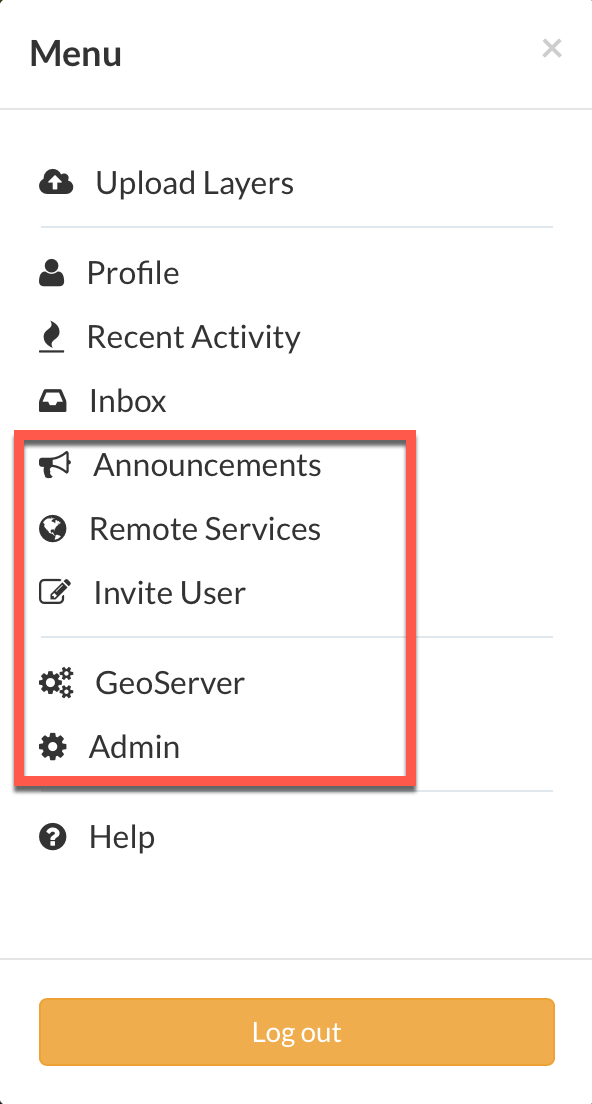
\includegraphics[width=8cm]{Images/admin_menu1.png}
	\caption{Admin menu entries}\label{fig:admin_menu1}
\end{figure}

\subsection{Adding users to groups}

Users who created a group or were made manager of a group can make other users members of that group.

\begin{figure}[H]
	\centering
	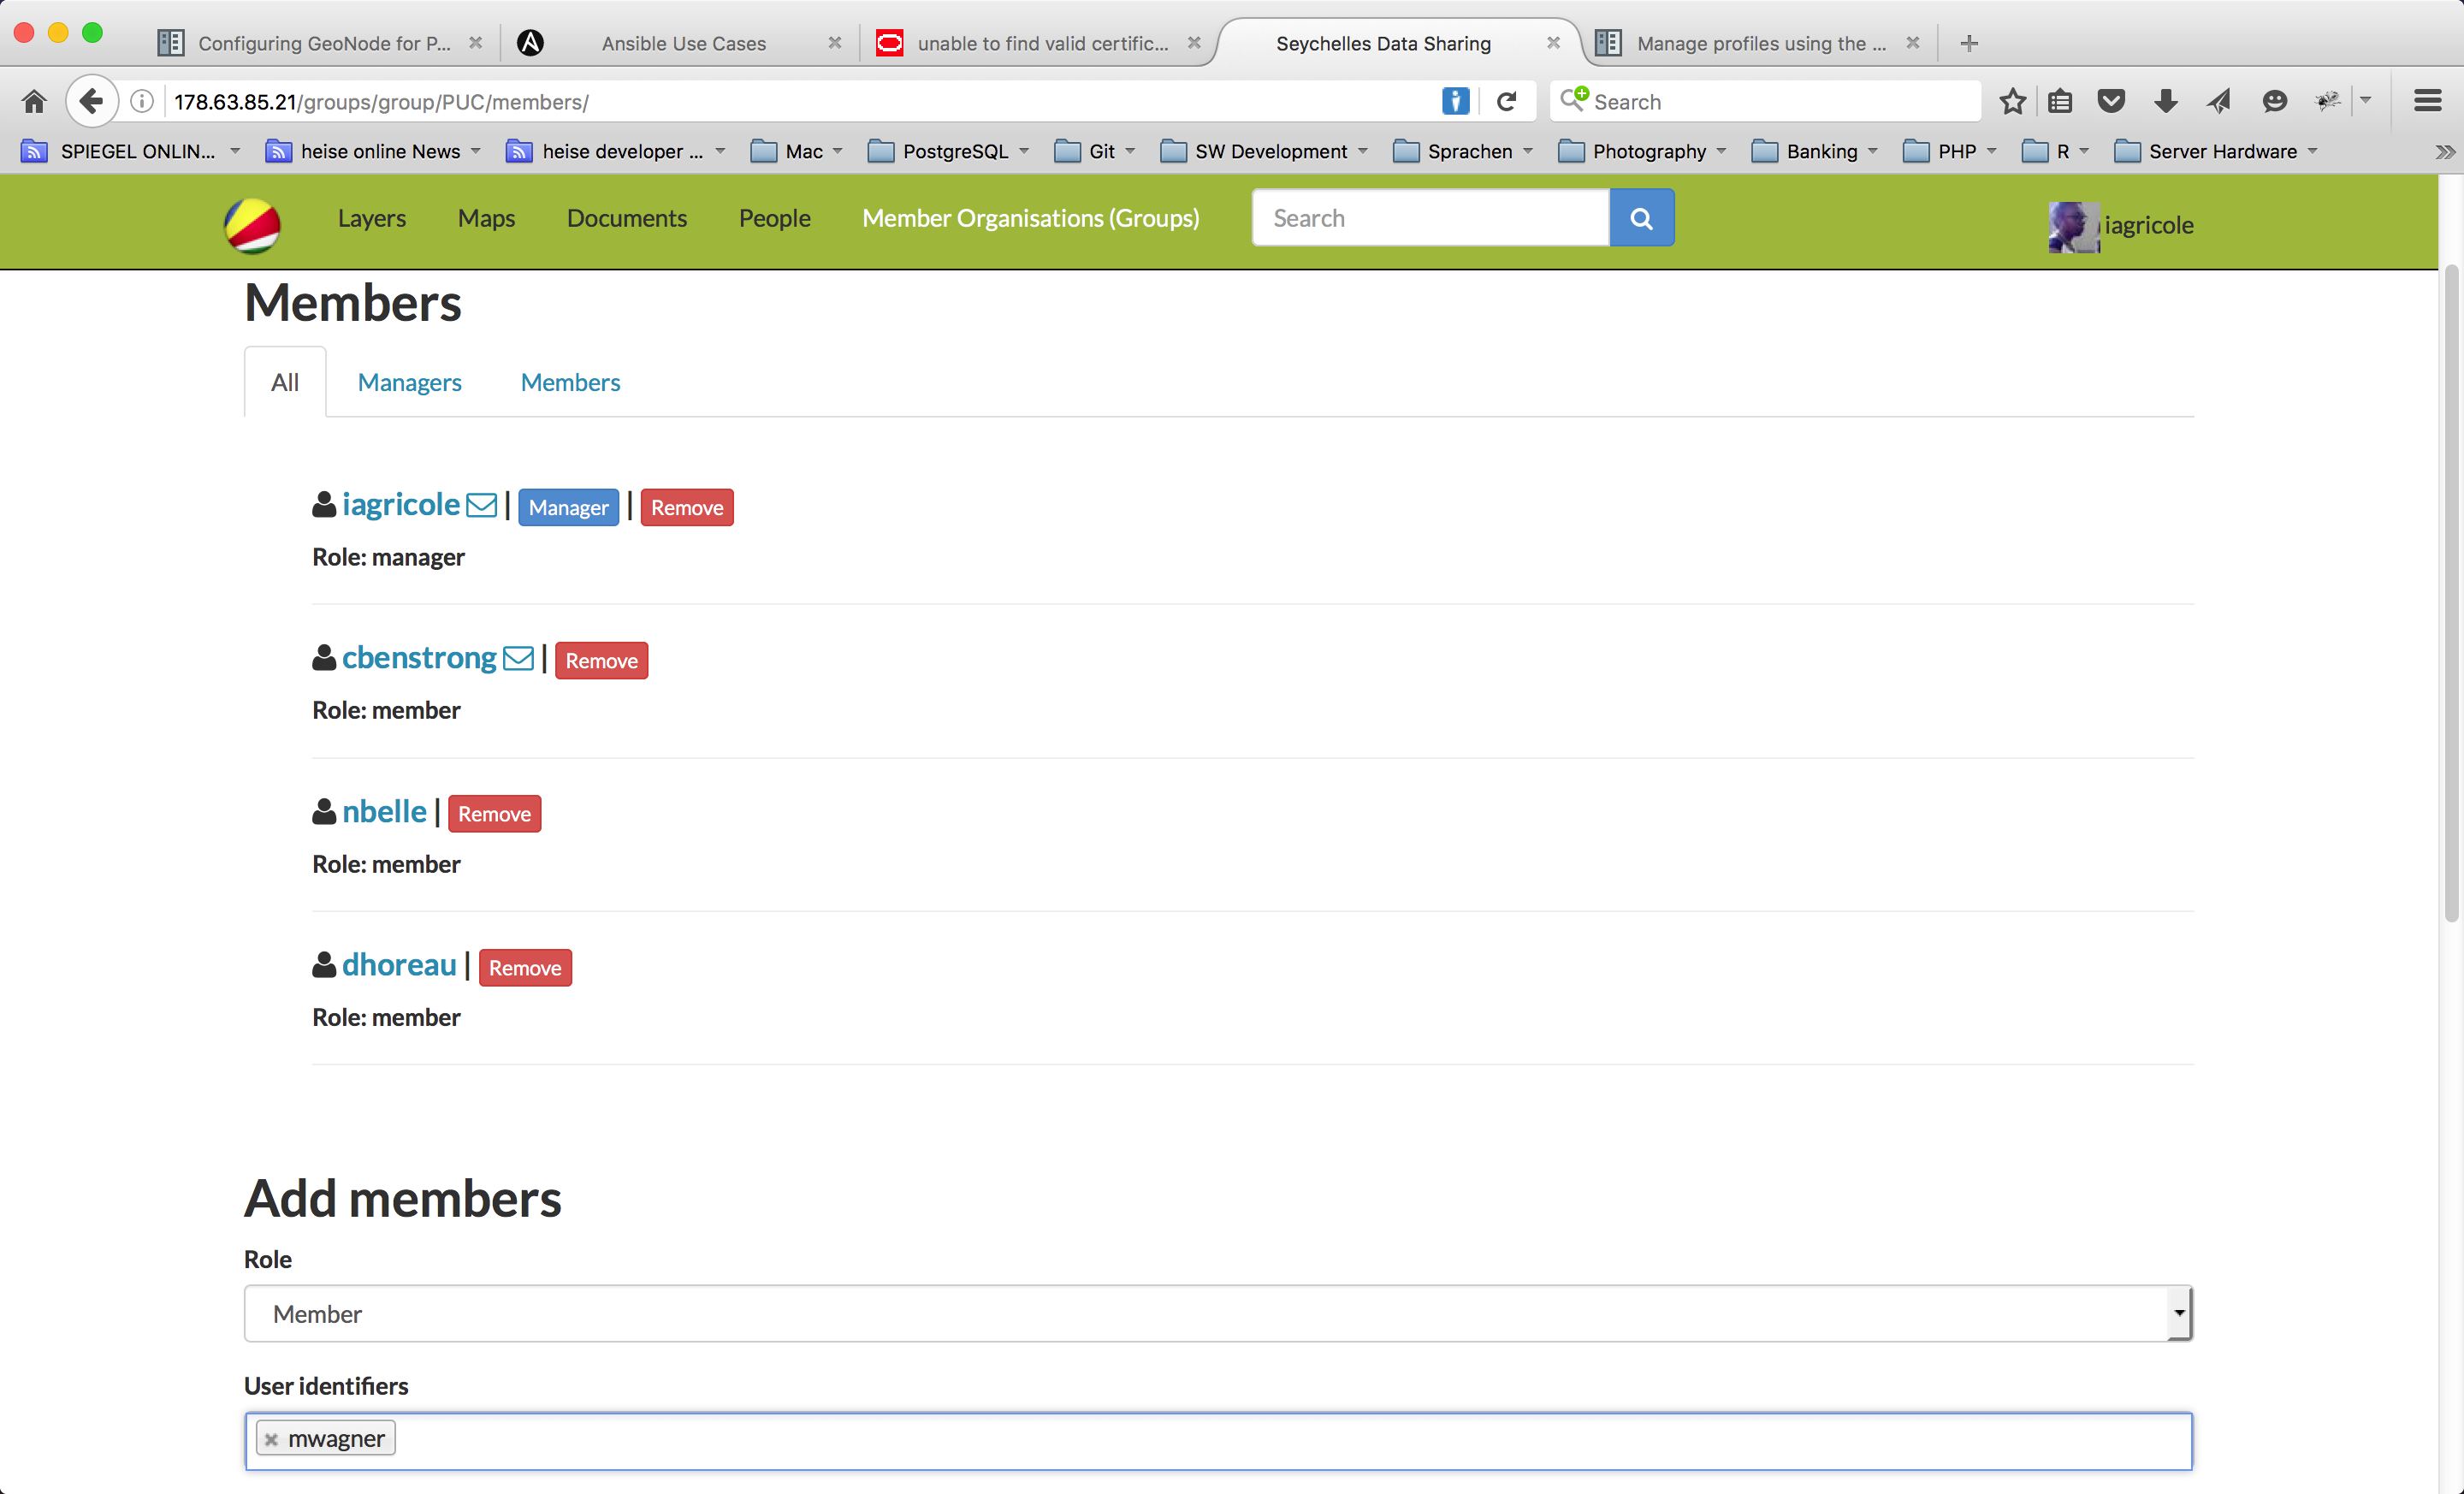
\includegraphics[width=12cm]{Images/add_user_to_group.png}
	\caption{Adding a user to a group}\label{fig:add_user_to_group}
\end{figure}


\subsection{Announcements}

Announcements can be used to inform the GeoNode users about upcoming maintenance work for example (Figure \ref{fig:announcement}).

\begin{figure}[H]
	\centering
	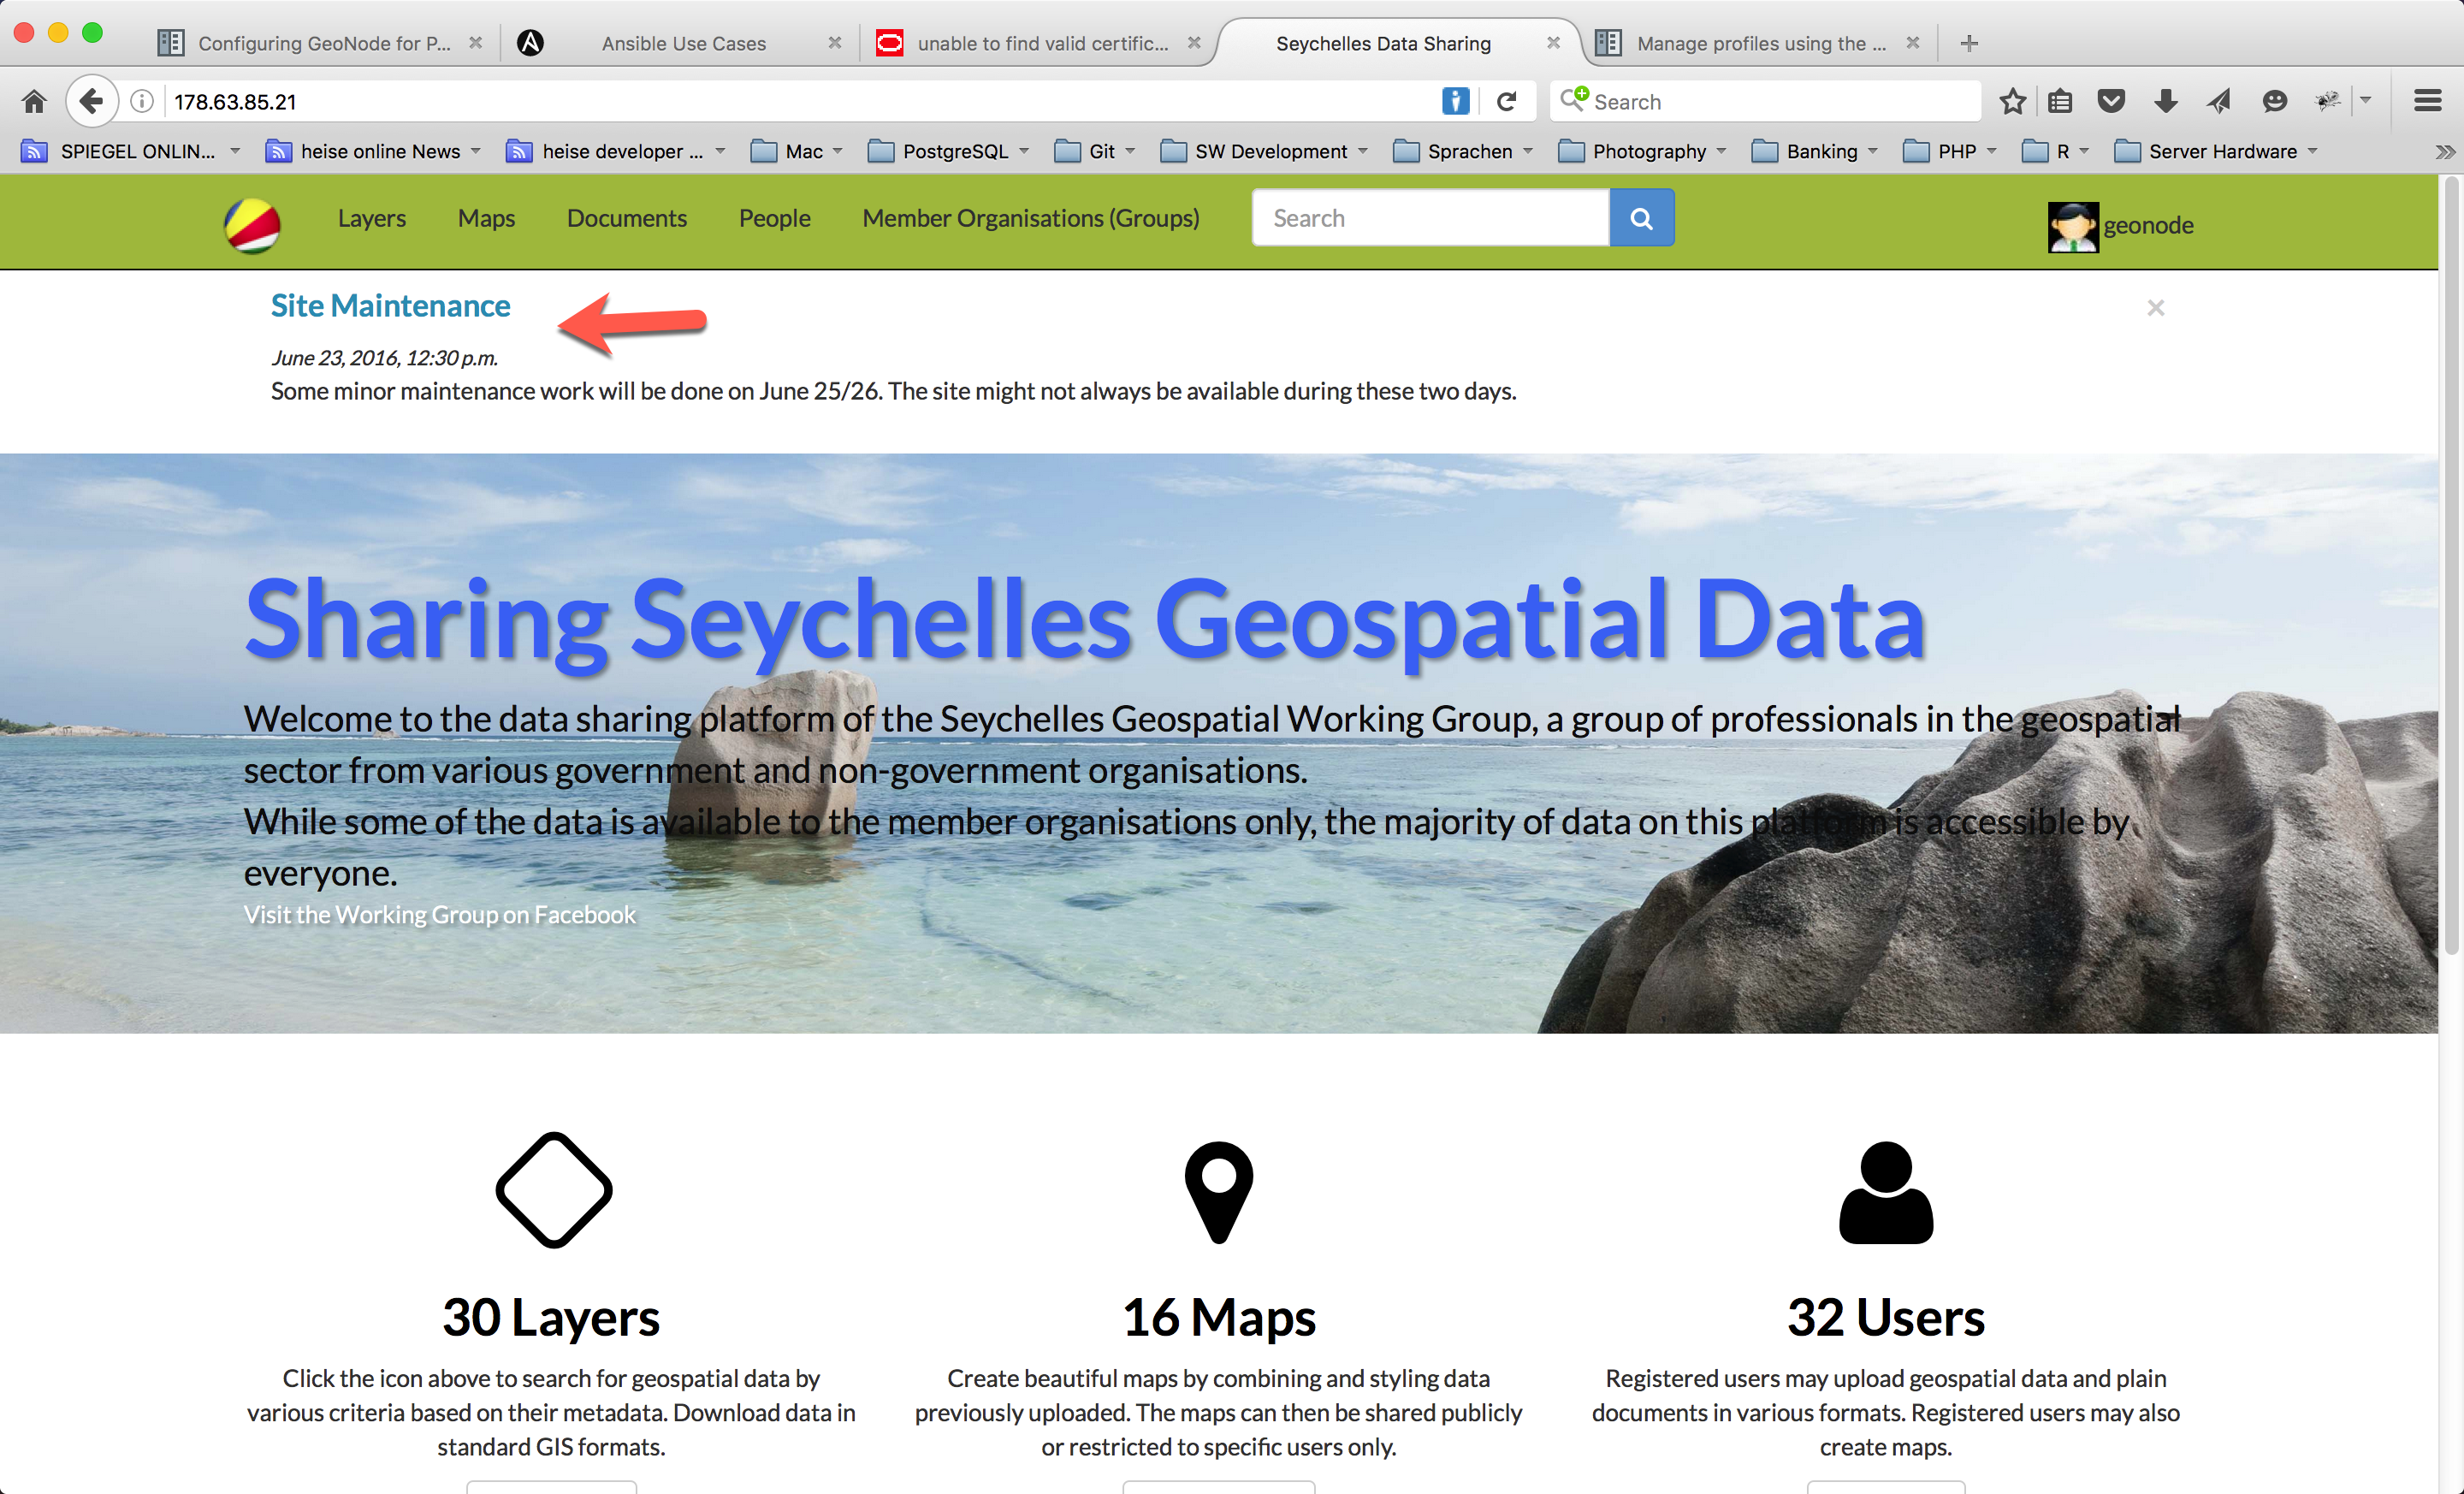
\includegraphics[width=12cm]{Images/announcement.png}
	\caption{Announcement}\label{fig:announcement}
\end{figure}

When creating an announcement a period of time can be defined for its publishing and the announcement will be shown only within that period.

\subsection{Remote Services}

A web service (e.g. WMS) and the relating layers can be registered via this option (Figure \ref{fig:register_service}). It is important that the web service supports the coordinate reference system with EPSG:ID 900913.

\begin{figure}[H]
	\centering
	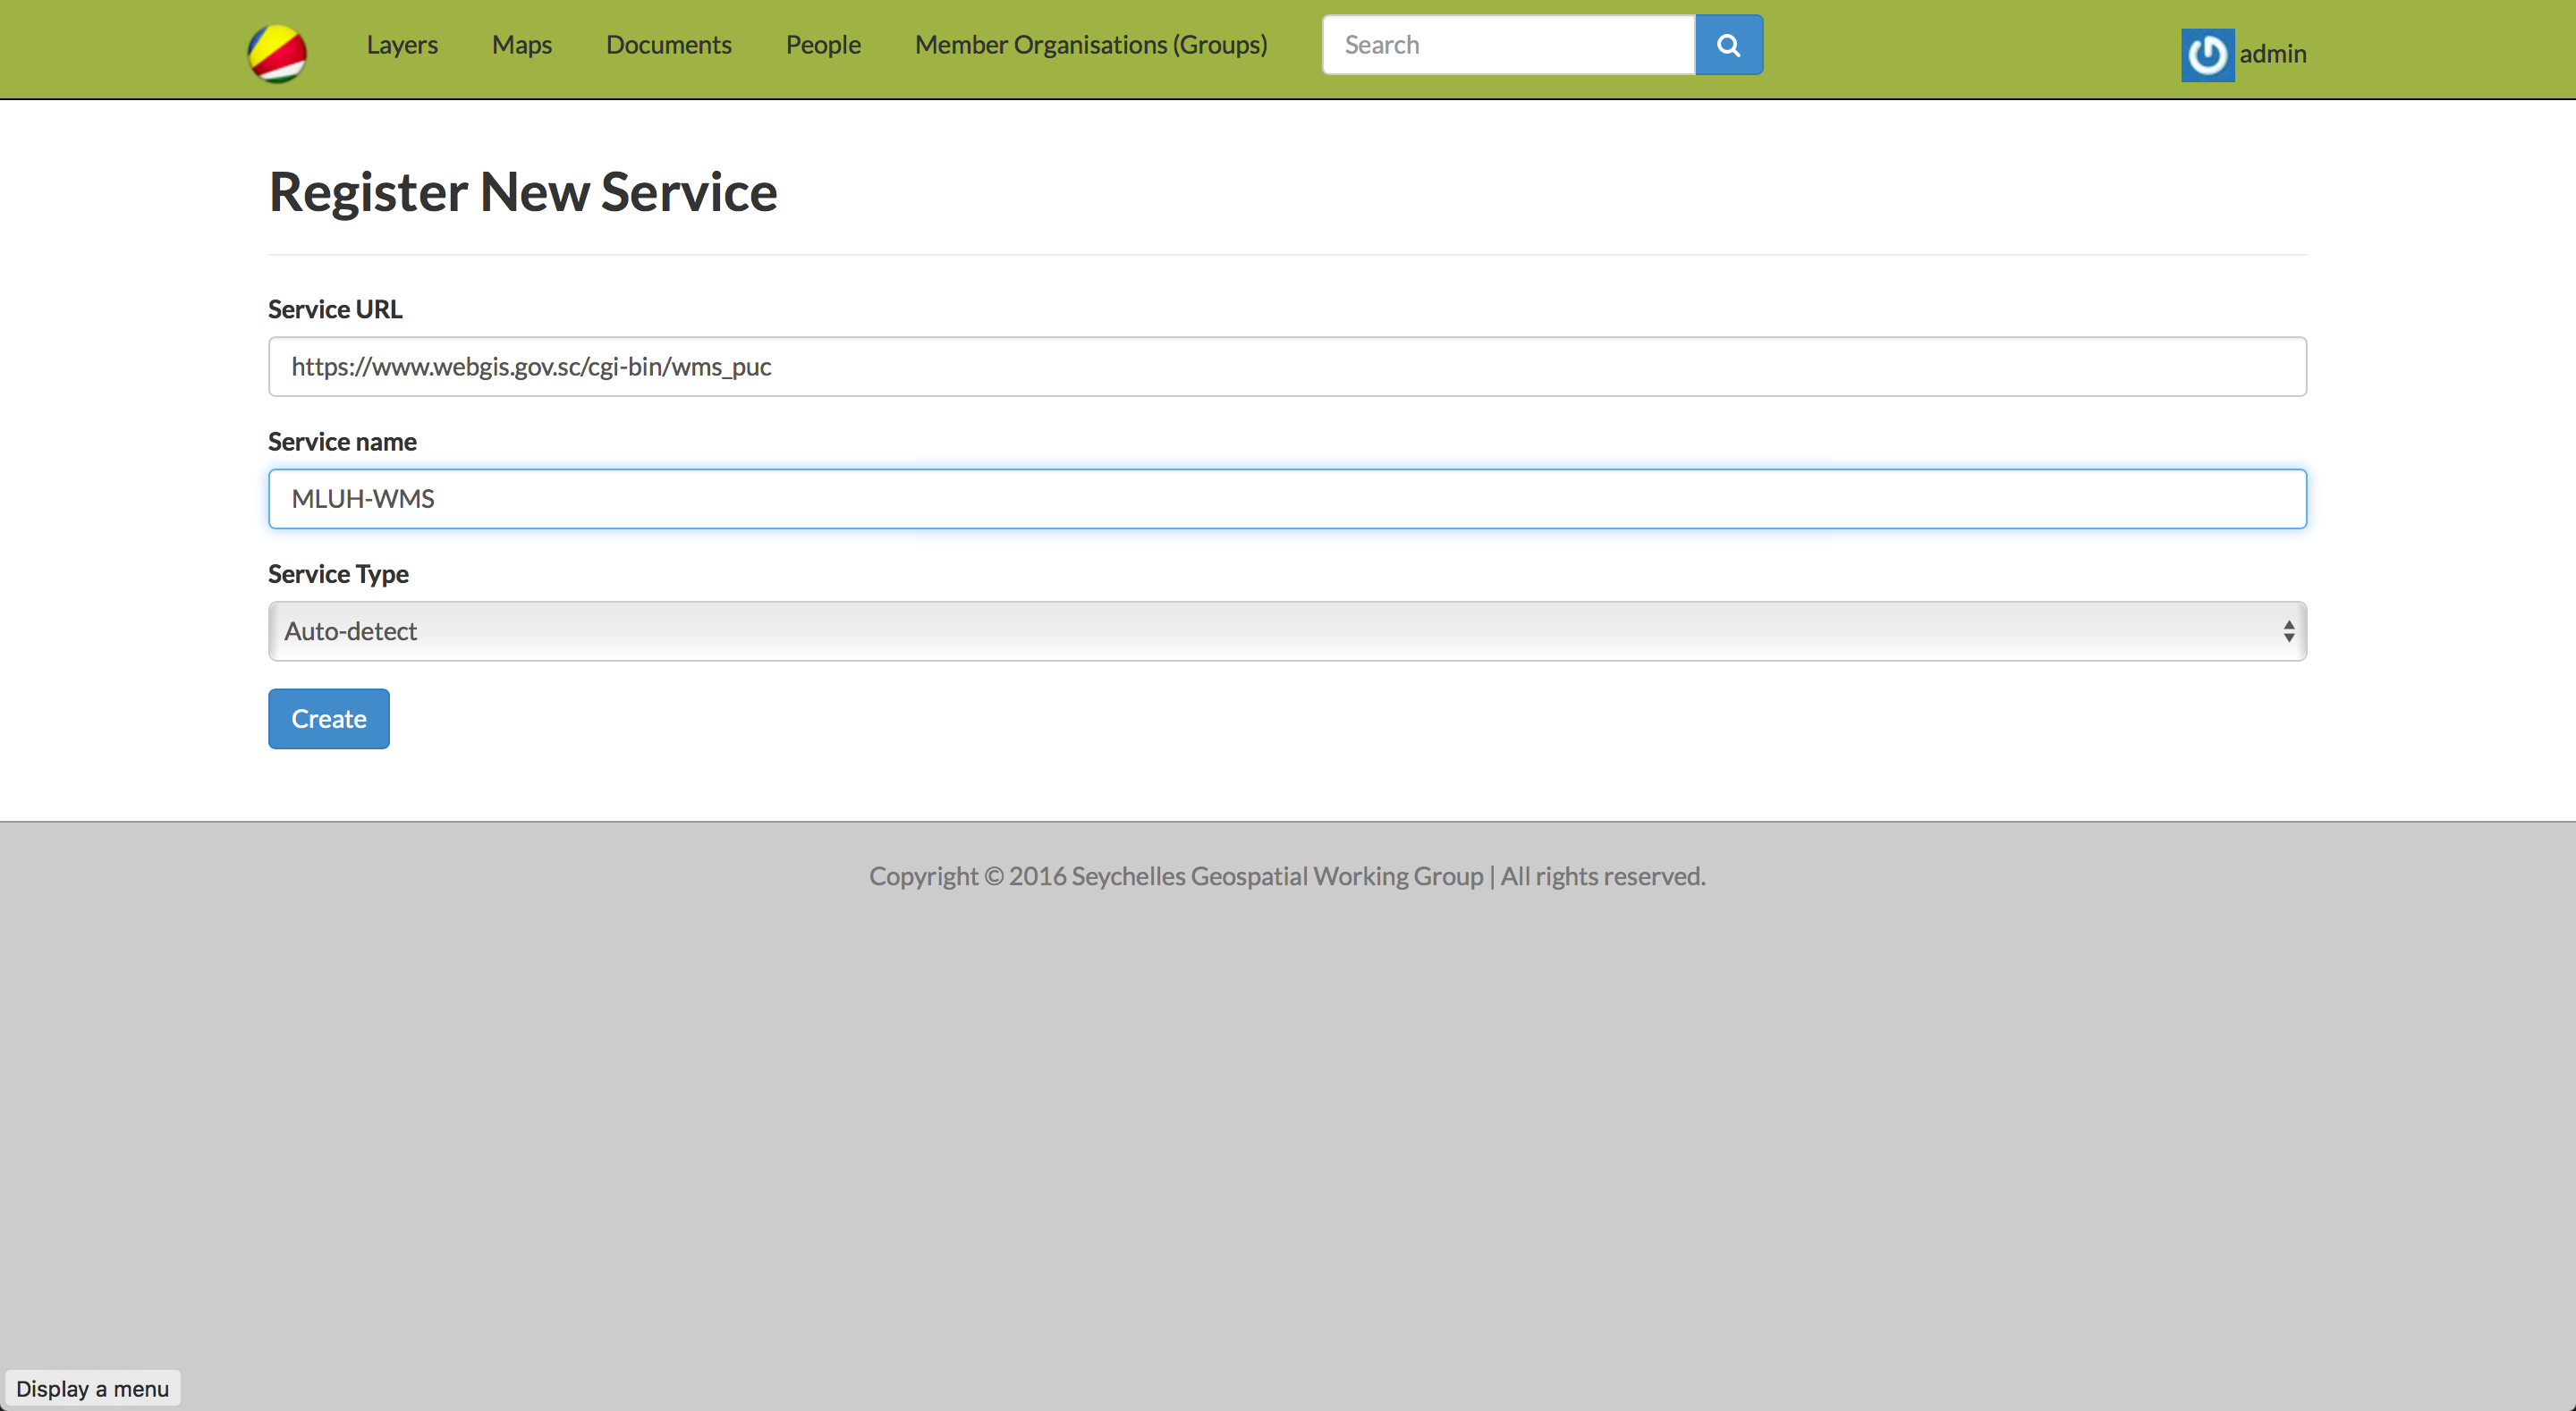
\includegraphics[width=12cm]{Images/register_service.png}
	\caption{Registering a remote service}\label{fig:register_service}
\end{figure}

On success the layers provided by the service will be added to the list of layers in GeoNode and can then be used to build a map.

\subsection{Admin}

This is where most of the GeoNode administration and any kind of bulk operation can be done, e.g. deleting several layers at once, etc. A lot of care should be taken when working in this section.

\begin{figure}[H]
	\centering
	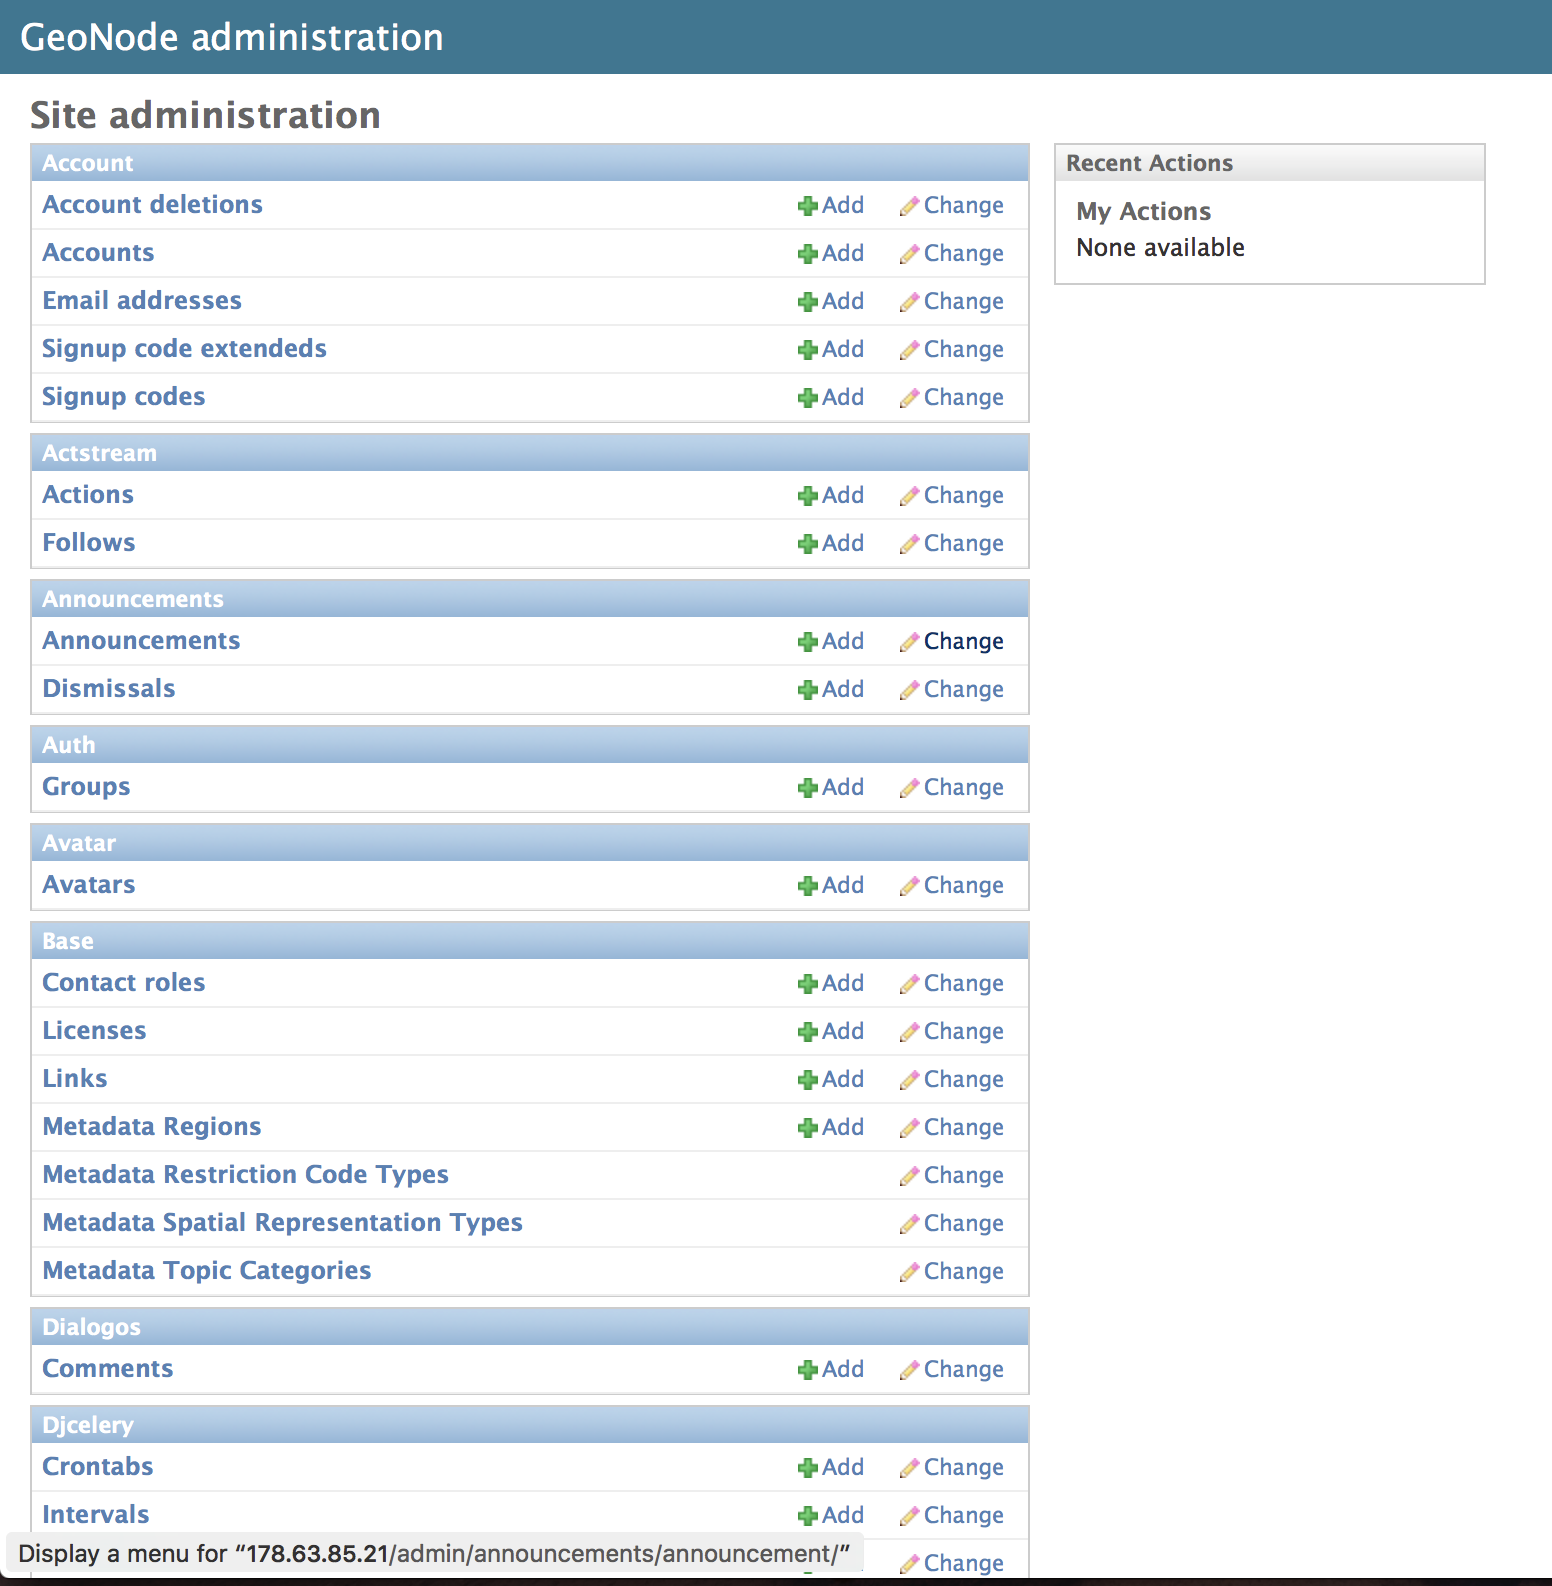
\includegraphics[width=8cm]{Images/geonode_admin.png}
	\caption{GeoNode Administration Area}\label{fig:geonode_admin}
\end{figure}

Create a new user from within that section (People:Users:Add) as shown in Figure \ref{fig:add_user}.

\begin{figure}[H]
	\centering
	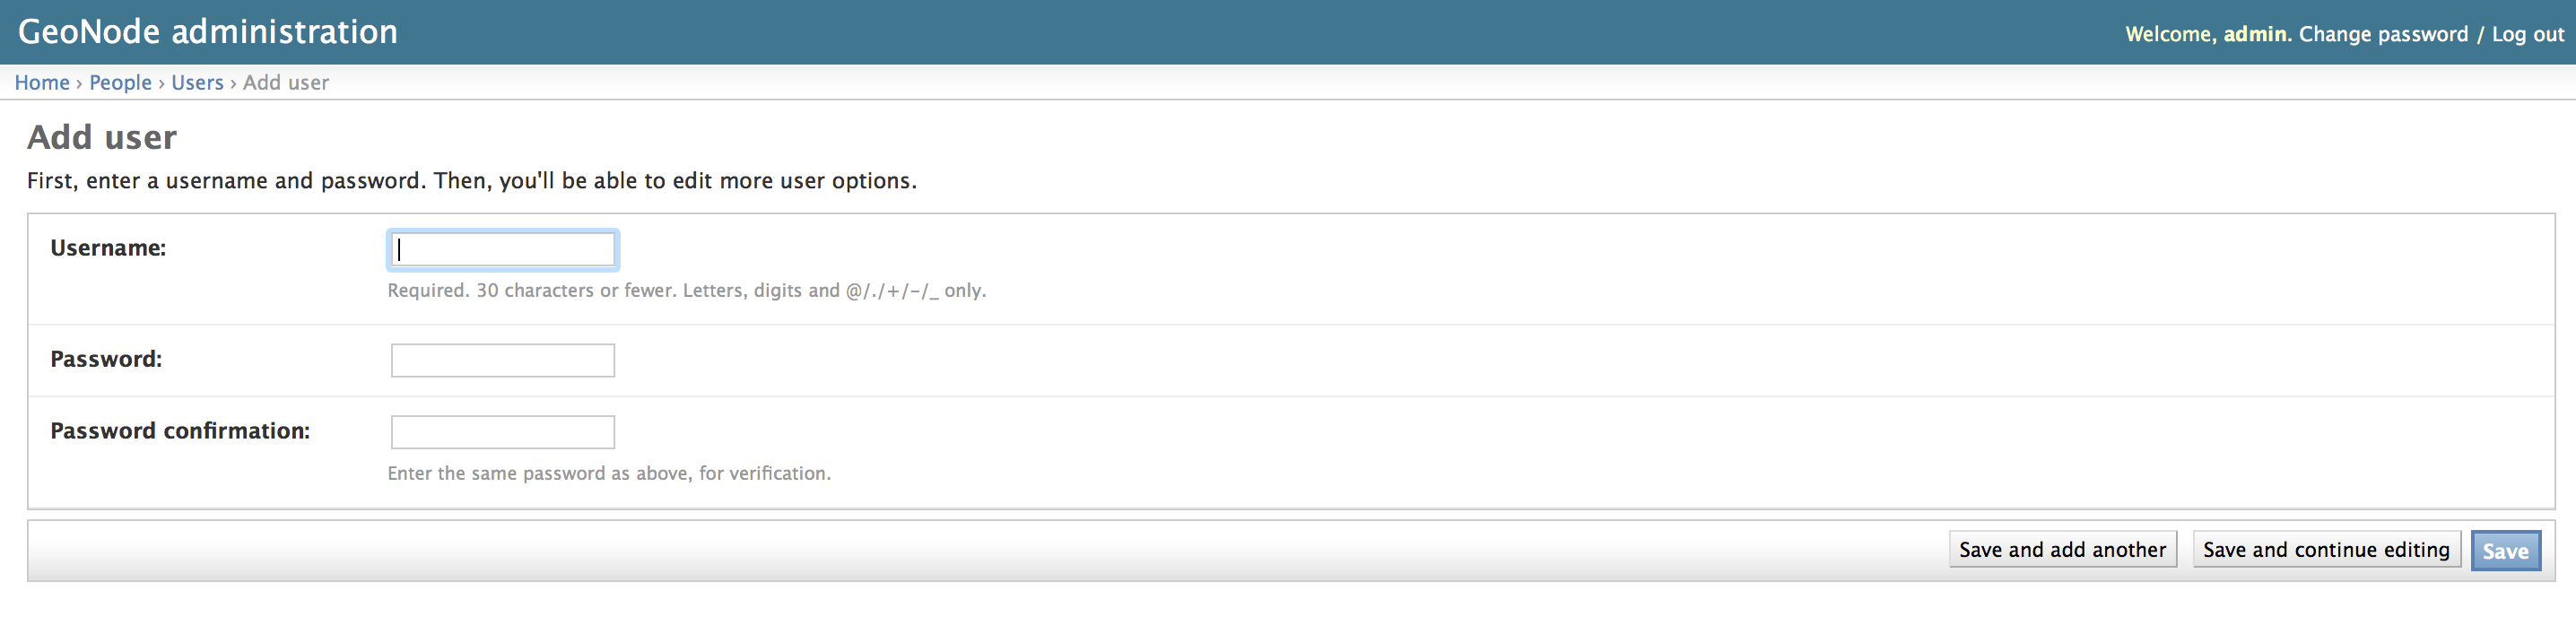
\includegraphics[width=8cm]{Images/add_user.png}
	\caption{Adding a new user}\label{fig:add_user}
\end{figure}

\end{document}
